% Options for packages loaded elsewhere
\PassOptionsToPackage{unicode}{hyperref}
\PassOptionsToPackage{hyphens}{url}
%
\documentclass[
]{article}
\usepackage{amsmath,amssymb}
\usepackage{iftex}
\ifPDFTeX
  \usepackage[T1]{fontenc}
  \usepackage[utf8]{inputenc}
  \usepackage{textcomp} % provide euro and other symbols
\else % if luatex or xetex
  \usepackage{unicode-math} % this also loads fontspec
  \defaultfontfeatures{Scale=MatchLowercase}
  \defaultfontfeatures[\rmfamily]{Ligatures=TeX,Scale=1}
\fi
\usepackage{lmodern}
\ifPDFTeX\else
  % xetex/luatex font selection
\fi
% Use upquote if available, for straight quotes in verbatim environments
\IfFileExists{upquote.sty}{\usepackage{upquote}}{}
\IfFileExists{microtype.sty}{% use microtype if available
  \usepackage[]{microtype}
  \UseMicrotypeSet[protrusion]{basicmath} % disable protrusion for tt fonts
}{}
\makeatletter
\@ifundefined{KOMAClassName}{% if non-KOMA class
  \IfFileExists{parskip.sty}{%
    \usepackage{parskip}
  }{% else
    \setlength{\parindent}{0pt}
    \setlength{\parskip}{6pt plus 2pt minus 1pt}}
}{% if KOMA class
  \KOMAoptions{parskip=half}}
\makeatother
\usepackage{xcolor}
\usepackage[margin=1in]{geometry}
\usepackage{color}
\usepackage{fancyvrb}
\newcommand{\VerbBar}{|}
\newcommand{\VERB}{\Verb[commandchars=\\\{\}]}
\DefineVerbatimEnvironment{Highlighting}{Verbatim}{commandchars=\\\{\}}
% Add ',fontsize=\small' for more characters per line
\usepackage{framed}
\definecolor{shadecolor}{RGB}{248,248,248}
\newenvironment{Shaded}{\begin{snugshade}}{\end{snugshade}}
\newcommand{\AlertTok}[1]{\textcolor[rgb]{0.94,0.16,0.16}{#1}}
\newcommand{\AnnotationTok}[1]{\textcolor[rgb]{0.56,0.35,0.01}{\textbf{\textit{#1}}}}
\newcommand{\AttributeTok}[1]{\textcolor[rgb]{0.13,0.29,0.53}{#1}}
\newcommand{\BaseNTok}[1]{\textcolor[rgb]{0.00,0.00,0.81}{#1}}
\newcommand{\BuiltInTok}[1]{#1}
\newcommand{\CharTok}[1]{\textcolor[rgb]{0.31,0.60,0.02}{#1}}
\newcommand{\CommentTok}[1]{\textcolor[rgb]{0.56,0.35,0.01}{\textit{#1}}}
\newcommand{\CommentVarTok}[1]{\textcolor[rgb]{0.56,0.35,0.01}{\textbf{\textit{#1}}}}
\newcommand{\ConstantTok}[1]{\textcolor[rgb]{0.56,0.35,0.01}{#1}}
\newcommand{\ControlFlowTok}[1]{\textcolor[rgb]{0.13,0.29,0.53}{\textbf{#1}}}
\newcommand{\DataTypeTok}[1]{\textcolor[rgb]{0.13,0.29,0.53}{#1}}
\newcommand{\DecValTok}[1]{\textcolor[rgb]{0.00,0.00,0.81}{#1}}
\newcommand{\DocumentationTok}[1]{\textcolor[rgb]{0.56,0.35,0.01}{\textbf{\textit{#1}}}}
\newcommand{\ErrorTok}[1]{\textcolor[rgb]{0.64,0.00,0.00}{\textbf{#1}}}
\newcommand{\ExtensionTok}[1]{#1}
\newcommand{\FloatTok}[1]{\textcolor[rgb]{0.00,0.00,0.81}{#1}}
\newcommand{\FunctionTok}[1]{\textcolor[rgb]{0.13,0.29,0.53}{\textbf{#1}}}
\newcommand{\ImportTok}[1]{#1}
\newcommand{\InformationTok}[1]{\textcolor[rgb]{0.56,0.35,0.01}{\textbf{\textit{#1}}}}
\newcommand{\KeywordTok}[1]{\textcolor[rgb]{0.13,0.29,0.53}{\textbf{#1}}}
\newcommand{\NormalTok}[1]{#1}
\newcommand{\OperatorTok}[1]{\textcolor[rgb]{0.81,0.36,0.00}{\textbf{#1}}}
\newcommand{\OtherTok}[1]{\textcolor[rgb]{0.56,0.35,0.01}{#1}}
\newcommand{\PreprocessorTok}[1]{\textcolor[rgb]{0.56,0.35,0.01}{\textit{#1}}}
\newcommand{\RegionMarkerTok}[1]{#1}
\newcommand{\SpecialCharTok}[1]{\textcolor[rgb]{0.81,0.36,0.00}{\textbf{#1}}}
\newcommand{\SpecialStringTok}[1]{\textcolor[rgb]{0.31,0.60,0.02}{#1}}
\newcommand{\StringTok}[1]{\textcolor[rgb]{0.31,0.60,0.02}{#1}}
\newcommand{\VariableTok}[1]{\textcolor[rgb]{0.00,0.00,0.00}{#1}}
\newcommand{\VerbatimStringTok}[1]{\textcolor[rgb]{0.31,0.60,0.02}{#1}}
\newcommand{\WarningTok}[1]{\textcolor[rgb]{0.56,0.35,0.01}{\textbf{\textit{#1}}}}
\usepackage{longtable,booktabs,array}
\usepackage{calc} % for calculating minipage widths
% Correct order of tables after \paragraph or \subparagraph
\usepackage{etoolbox}
\makeatletter
\patchcmd\longtable{\par}{\if@noskipsec\mbox{}\fi\par}{}{}
\makeatother
% Allow footnotes in longtable head/foot
\IfFileExists{footnotehyper.sty}{\usepackage{footnotehyper}}{\usepackage{footnote}}
\makesavenoteenv{longtable}
\usepackage{graphicx}
\makeatletter
\def\maxwidth{\ifdim\Gin@nat@width>\linewidth\linewidth\else\Gin@nat@width\fi}
\def\maxheight{\ifdim\Gin@nat@height>\textheight\textheight\else\Gin@nat@height\fi}
\makeatother
% Scale images if necessary, so that they will not overflow the page
% margins by default, and it is still possible to overwrite the defaults
% using explicit options in \includegraphics[width, height, ...]{}
\setkeys{Gin}{width=\maxwidth,height=\maxheight,keepaspectratio}
% Set default figure placement to htbp
\makeatletter
\def\fps@figure{htbp}
\makeatother
\setlength{\emergencystretch}{3em} % prevent overfull lines
\providecommand{\tightlist}{%
  \setlength{\itemsep}{0pt}\setlength{\parskip}{0pt}}
\setcounter{secnumdepth}{-\maxdimen} % remove section numbering
\ifLuaTeX
  \usepackage{selnolig}  % disable illegal ligatures
\fi
\usepackage{bookmark}
\IfFileExists{xurl.sty}{\usepackage{xurl}}{} % add URL line breaks if available
\urlstyle{same}
\hypersetup{
  pdftitle={P8106\_midterm\_project\_v1},
  pdfauthor={Congyu Yang, Yujing Fu, Zhengkun Ou},
  hidelinks,
  pdfcreator={LaTeX via pandoc}}

\title{P8106\_midterm\_project\_v1}
\author{Congyu Yang, Yujing Fu, Zhengkun Ou}
\date{2025-03-27}

\begin{document}
\maketitle

\begin{Shaded}
\begin{Highlighting}[]
\FunctionTok{library}\NormalTok{(pacman)}
\FunctionTok{p\_load}\NormalTok{(tidyverse, caret, tidymodels, corrplot, ggplot2, plotmo, ggrepel, patchwork, earth, pdp, mgcv, knitr)}
\end{Highlighting}
\end{Shaded}

\begin{verbatim}
## package 'cli' successfully unpacked and MD5 sums checked
\end{verbatim}

\begin{verbatim}
## package 'purrr' successfully unpacked and MD5 sums checked
\end{verbatim}

\begin{verbatim}
## package 'rlang' successfully unpacked and MD5 sums checked
\end{verbatim}

\begin{verbatim}
## package 'tidymodels' successfully unpacked and MD5 sums checked
## 
## The downloaded binary packages are in
##  C:\Users\Persica\AppData\Local\Temp\RtmpOo34bM\downloaded_packages
\end{verbatim}

\subsection{1. Data Processing}\label{data-processing}

\begin{Shaded}
\begin{Highlighting}[]
\FunctionTok{load}\NormalTok{(}\StringTok{"dat1.RData"}\NormalTok{)}
\FunctionTok{load}\NormalTok{(}\StringTok{"dat2.RData"}\NormalTok{)}
\end{Highlighting}
\end{Shaded}

\begin{Shaded}
\begin{Highlighting}[]
\NormalTok{skimr}\SpecialCharTok{::}\FunctionTok{skim}\NormalTok{(dat1)}
\end{Highlighting}
\end{Shaded}

\begin{longtable}[]{@{}ll@{}}
\caption{Data summary}\tabularnewline
\toprule\noalign{}
\endfirsthead
\endhead
\bottomrule\noalign{}
\endlastfoot
Name & dat1 \\
Number of rows & 5000 \\
Number of columns & 14 \\
\_\_\_\_\_\_\_\_\_\_\_\_\_\_\_\_\_\_\_\_\_\_\_ & \\
Column type frequency: & \\
factor & 2 \\
numeric & 12 \\
\_\_\_\_\_\_\_\_\_\_\_\_\_\_\_\_\_\_\_\_\_\_\_\_ & \\
Group variables & None \\
\end{longtable}

\textbf{Variable type: factor}

\begin{longtable}[]{@{}
  >{\raggedright\arraybackslash}p{(\columnwidth - 10\tabcolsep) * \real{0.1591}}
  >{\raggedleft\arraybackslash}p{(\columnwidth - 10\tabcolsep) * \real{0.1136}}
  >{\raggedleft\arraybackslash}p{(\columnwidth - 10\tabcolsep) * \real{0.1591}}
  >{\raggedright\arraybackslash}p{(\columnwidth - 10\tabcolsep) * \real{0.0909}}
  >{\raggedleft\arraybackslash}p{(\columnwidth - 10\tabcolsep) * \real{0.1023}}
  >{\raggedright\arraybackslash}p{(\columnwidth - 10\tabcolsep) * \real{0.3750}}@{}}
\toprule\noalign{}
\begin{minipage}[b]{\linewidth}\raggedright
skim\_variable
\end{minipage} & \begin{minipage}[b]{\linewidth}\raggedleft
n\_missing
\end{minipage} & \begin{minipage}[b]{\linewidth}\raggedleft
complete\_rate
\end{minipage} & \begin{minipage}[b]{\linewidth}\raggedright
ordered
\end{minipage} & \begin{minipage}[b]{\linewidth}\raggedleft
n\_unique
\end{minipage} & \begin{minipage}[b]{\linewidth}\raggedright
top\_counts
\end{minipage} \\
\midrule\noalign{}
\endhead
\bottomrule\noalign{}
\endlastfoot
race & 0 & 1 & FALSE & 4 & 1: 3221, 3: 1036, 4: 465, 2: 278 \\
smoking & 0 & 1 & FALSE & 3 & 0: 3010, 1: 1504, 2: 486 \\
\end{longtable}

\textbf{Variable type: numeric}

\begin{longtable}[]{@{}
  >{\raggedright\arraybackslash}p{(\columnwidth - 20\tabcolsep) * \real{0.1414}}
  >{\raggedleft\arraybackslash}p{(\columnwidth - 20\tabcolsep) * \real{0.1010}}
  >{\raggedleft\arraybackslash}p{(\columnwidth - 20\tabcolsep) * \real{0.1414}}
  >{\raggedleft\arraybackslash}p{(\columnwidth - 20\tabcolsep) * \real{0.0808}}
  >{\raggedleft\arraybackslash}p{(\columnwidth - 20\tabcolsep) * \real{0.0808}}
  >{\raggedleft\arraybackslash}p{(\columnwidth - 20\tabcolsep) * \real{0.0707}}
  >{\raggedleft\arraybackslash}p{(\columnwidth - 20\tabcolsep) * \real{0.0808}}
  >{\raggedleft\arraybackslash}p{(\columnwidth - 20\tabcolsep) * \real{0.0808}}
  >{\raggedleft\arraybackslash}p{(\columnwidth - 20\tabcolsep) * \real{0.0808}}
  >{\raggedleft\arraybackslash}p{(\columnwidth - 20\tabcolsep) * \real{0.0808}}
  >{\raggedright\arraybackslash}p{(\columnwidth - 20\tabcolsep) * \real{0.0606}}@{}}
\toprule\noalign{}
\begin{minipage}[b]{\linewidth}\raggedright
skim\_variable
\end{minipage} & \begin{minipage}[b]{\linewidth}\raggedleft
n\_missing
\end{minipage} & \begin{minipage}[b]{\linewidth}\raggedleft
complete\_rate
\end{minipage} & \begin{minipage}[b]{\linewidth}\raggedleft
mean
\end{minipage} & \begin{minipage}[b]{\linewidth}\raggedleft
sd
\end{minipage} & \begin{minipage}[b]{\linewidth}\raggedleft
p0
\end{minipage} & \begin{minipage}[b]{\linewidth}\raggedleft
p25
\end{minipage} & \begin{minipage}[b]{\linewidth}\raggedleft
p50
\end{minipage} & \begin{minipage}[b]{\linewidth}\raggedleft
p75
\end{minipage} & \begin{minipage}[b]{\linewidth}\raggedleft
p100
\end{minipage} & \begin{minipage}[b]{\linewidth}\raggedright
hist
\end{minipage} \\
\midrule\noalign{}
\endhead
\bottomrule\noalign{}
\endlastfoot
id & 0 & 1 & 2500.50 & 1443.52 & 1.00 & 1250.75 & 2500.50 & 3750.25 &
5000.00 & ▇▇▇▇▇ \\
age & 0 & 1 & 59.97 & 4.50 & 44.00 & 57.00 & 60.00 & 63.00 & 75.00 &
▁▃▇▅▁ \\
gender & 0 & 1 & 0.49 & 0.50 & 0.00 & 0.00 & 0.00 & 1.00 & 1.00 &
▇▁▁▁▇ \\
height & 0 & 1 & 170.13 & 5.94 & 150.20 & 166.10 & 170.10 & 174.22 &
192.90 & ▁▅▇▂▁ \\
weight & 0 & 1 & 80.11 & 7.06 & 56.70 & 75.40 & 80.10 & 84.90 & 106.00 &
▁▅▇▃▁ \\
bmi & 0 & 1 & 27.74 & 2.76 & 18.20 & 25.80 & 27.60 & 29.50 & 38.80 &
▁▅▇▂▁ \\
diabetes & 0 & 1 & 0.15 & 0.36 & 0.00 & 0.00 & 0.00 & 0.00 & 1.00 &
▇▁▁▁▂ \\
hypertension & 0 & 1 & 0.46 & 0.50 & 0.00 & 0.00 & 0.00 & 1.00 & 1.00 &
▇▁▁▁▇ \\
SBP & 0 & 1 & 129.90 & 8.00 & 101.00 & 124.00 & 130.00 & 135.00 & 155.00
& ▁▂▇▅▁ \\
LDL & 0 & 1 & 109.91 & 20.15 & 43.00 & 96.00 & 110.00 & 124.00 & 185.00
& ▁▅▇▂▁ \\
time & 0 & 1 & 108.86 & 43.42 & 30.00 & 76.00 & 106.00 & 138.00 & 270.00
& ▆▇▅▂▁ \\
log\_antibody & 0 & 1 & 10.06 & 0.60 & 7.77 & 9.68 & 10.09 & 10.48 &
11.96 & ▁▂▇▆▁ \\
\end{longtable}

\begin{Shaded}
\begin{Highlighting}[]
\NormalTok{skimr}\SpecialCharTok{::}\FunctionTok{skim}\NormalTok{(dat2)}
\end{Highlighting}
\end{Shaded}

\begin{longtable}[]{@{}ll@{}}
\caption{Data summary}\tabularnewline
\toprule\noalign{}
\endfirsthead
\endhead
\bottomrule\noalign{}
\endlastfoot
Name & dat2 \\
Number of rows & 1000 \\
Number of columns & 14 \\
\_\_\_\_\_\_\_\_\_\_\_\_\_\_\_\_\_\_\_\_\_\_\_ & \\
Column type frequency: & \\
factor & 2 \\
numeric & 12 \\
\_\_\_\_\_\_\_\_\_\_\_\_\_\_\_\_\_\_\_\_\_\_\_\_ & \\
Group variables & None \\
\end{longtable}

\textbf{Variable type: factor}

\begin{longtable}[]{@{}
  >{\raggedright\arraybackslash}p{(\columnwidth - 10\tabcolsep) * \real{0.1667}}
  >{\raggedleft\arraybackslash}p{(\columnwidth - 10\tabcolsep) * \real{0.1190}}
  >{\raggedleft\arraybackslash}p{(\columnwidth - 10\tabcolsep) * \real{0.1667}}
  >{\raggedright\arraybackslash}p{(\columnwidth - 10\tabcolsep) * \real{0.0952}}
  >{\raggedleft\arraybackslash}p{(\columnwidth - 10\tabcolsep) * \real{0.1071}}
  >{\raggedright\arraybackslash}p{(\columnwidth - 10\tabcolsep) * \real{0.3452}}@{}}
\toprule\noalign{}
\begin{minipage}[b]{\linewidth}\raggedright
skim\_variable
\end{minipage} & \begin{minipage}[b]{\linewidth}\raggedleft
n\_missing
\end{minipage} & \begin{minipage}[b]{\linewidth}\raggedleft
complete\_rate
\end{minipage} & \begin{minipage}[b]{\linewidth}\raggedright
ordered
\end{minipage} & \begin{minipage}[b]{\linewidth}\raggedleft
n\_unique
\end{minipage} & \begin{minipage}[b]{\linewidth}\raggedright
top\_counts
\end{minipage} \\
\midrule\noalign{}
\endhead
\bottomrule\noalign{}
\endlastfoot
race & 0 & 1 & FALSE & 4 & 1: 663, 3: 199, 4: 83, 2: 55 \\
smoking & 0 & 1 & FALSE & 3 & 0: 601, 1: 296, 2: 103 \\
\end{longtable}

\textbf{Variable type: numeric}

\begin{longtable}[]{@{}
  >{\raggedright\arraybackslash}p{(\columnwidth - 20\tabcolsep) * \real{0.1414}}
  >{\raggedleft\arraybackslash}p{(\columnwidth - 20\tabcolsep) * \real{0.1010}}
  >{\raggedleft\arraybackslash}p{(\columnwidth - 20\tabcolsep) * \real{0.1414}}
  >{\raggedleft\arraybackslash}p{(\columnwidth - 20\tabcolsep) * \real{0.0808}}
  >{\raggedleft\arraybackslash}p{(\columnwidth - 20\tabcolsep) * \real{0.0707}}
  >{\raggedleft\arraybackslash}p{(\columnwidth - 20\tabcolsep) * \real{0.0808}}
  >{\raggedleft\arraybackslash}p{(\columnwidth - 20\tabcolsep) * \real{0.0808}}
  >{\raggedleft\arraybackslash}p{(\columnwidth - 20\tabcolsep) * \real{0.0808}}
  >{\raggedleft\arraybackslash}p{(\columnwidth - 20\tabcolsep) * \real{0.0808}}
  >{\raggedleft\arraybackslash}p{(\columnwidth - 20\tabcolsep) * \real{0.0808}}
  >{\raggedright\arraybackslash}p{(\columnwidth - 20\tabcolsep) * \real{0.0606}}@{}}
\toprule\noalign{}
\begin{minipage}[b]{\linewidth}\raggedright
skim\_variable
\end{minipage} & \begin{minipage}[b]{\linewidth}\raggedleft
n\_missing
\end{minipage} & \begin{minipage}[b]{\linewidth}\raggedleft
complete\_rate
\end{minipage} & \begin{minipage}[b]{\linewidth}\raggedleft
mean
\end{minipage} & \begin{minipage}[b]{\linewidth}\raggedleft
sd
\end{minipage} & \begin{minipage}[b]{\linewidth}\raggedleft
p0
\end{minipage} & \begin{minipage}[b]{\linewidth}\raggedleft
p25
\end{minipage} & \begin{minipage}[b]{\linewidth}\raggedleft
p50
\end{minipage} & \begin{minipage}[b]{\linewidth}\raggedleft
p75
\end{minipage} & \begin{minipage}[b]{\linewidth}\raggedleft
p100
\end{minipage} & \begin{minipage}[b]{\linewidth}\raggedright
hist
\end{minipage} \\
\midrule\noalign{}
\endhead
\bottomrule\noalign{}
\endlastfoot
id & 0 & 1 & 5500.50 & 288.82 & 5001.00 & 5250.75 & 5500.50 & 5750.25 &
6000.00 & ▇▇▇▇▇ \\
age & 0 & 1 & 60.02 & 4.45 & 46.00 & 57.00 & 60.00 & 63.00 & 75.00 &
▁▃▇▃▁ \\
gender & 0 & 1 & 0.49 & 0.50 & 0.00 & 0.00 & 0.00 & 1.00 & 1.00 &
▇▁▁▁▇ \\
height & 0 & 1 & 170.22 & 6.02 & 149.40 & 166.10 & 170.20 & 174.20 &
190.60 & ▁▃▇▃▁ \\
weight & 0 & 1 & 80.13 & 7.05 & 58.80 & 75.30 & 80.20 & 84.40 & 101.60 &
▁▃▇▃▁ \\
bmi & 0 & 1 & 27.72 & 2.82 & 19.80 & 25.80 & 27.60 & 29.60 & 35.80 &
▁▅▇▃▁ \\
diabetes & 0 & 1 & 0.16 & 0.36 & 0.00 & 0.00 & 0.00 & 0.00 & 1.00 &
▇▁▁▁▂ \\
hypertension & 0 & 1 & 0.46 & 0.50 & 0.00 & 0.00 & 0.00 & 1.00 & 1.00 &
▇▁▁▁▇ \\
SBP & 0 & 1 & 129.61 & 8.20 & 106.00 & 124.00 & 130.00 & 135.00 & 156.00
& ▁▅▇▃▁ \\
LDL & 0 & 1 & 110.25 & 20.32 & 46.00 & 96.00 & 112.00 & 124.00 & 174.00
& ▁▅▇▅▁ \\
time & 0 & 1 & 173.77 & 46.78 & 61.00 & 140.00 & 171.00 & 205.00 &
330.00 & ▂▇▇▃▁ \\
log\_antibody & 0 & 1 & 9.90 & 0.59 & 8.05 & 9.50 & 9.93 & 10.31 & 11.85
& ▁▅▇▃▁ \\
\end{longtable}

There is no missing value in this dataset.

\begin{Shaded}
\begin{Highlighting}[]
\FunctionTok{colnames}\NormalTok{(dat1)}
\end{Highlighting}
\end{Shaded}

\begin{verbatim}
##  [1] "id"           "age"          "gender"       "race"         "smoking"     
##  [6] "height"       "weight"       "bmi"          "diabetes"     "hypertension"
## [11] "SBP"          "LDL"          "time"         "log_antibody"
\end{verbatim}

\begin{Shaded}
\begin{Highlighting}[]
\CommentTok{\# Clean variable names}
\NormalTok{dat1 }\OtherTok{=}\NormalTok{ dat1 }\SpecialCharTok{|\textgreater{}}\NormalTok{ janitor}\SpecialCharTok{::}\FunctionTok{clean\_names}\NormalTok{()}
\NormalTok{dat2 }\OtherTok{=}\NormalTok{ dat2 }\SpecialCharTok{|\textgreater{}}\NormalTok{ janitor}\SpecialCharTok{::}\FunctionTok{clean\_names}\NormalTok{()}
\end{Highlighting}
\end{Shaded}

We can see there is no NA values in the dataset.

\begin{Shaded}
\begin{Highlighting}[]
\CommentTok{\# Convert variables to factors}
\NormalTok{dat1}\SpecialCharTok{$}\NormalTok{gender }\OtherTok{\textless{}{-}} \FunctionTok{factor}\NormalTok{(dat1}\SpecialCharTok{$}\NormalTok{gender, }\AttributeTok{levels =} \FunctionTok{c}\NormalTok{(}\DecValTok{0}\NormalTok{, }\DecValTok{1}\NormalTok{), }\AttributeTok{labels =} \FunctionTok{c}\NormalTok{(}\StringTok{"Female"}\NormalTok{, }\StringTok{"Male"}\NormalTok{))}
\NormalTok{dat1}\SpecialCharTok{$}\NormalTok{race }\OtherTok{\textless{}{-}} \FunctionTok{factor}\NormalTok{(dat1}\SpecialCharTok{$}\NormalTok{race, }\AttributeTok{levels =} \FunctionTok{c}\NormalTok{(}\DecValTok{1}\NormalTok{, }\DecValTok{2}\NormalTok{, }\DecValTok{3}\NormalTok{, }\DecValTok{4}\NormalTok{), }\AttributeTok{labels =} \FunctionTok{c}\NormalTok{(}\StringTok{"White"}\NormalTok{, }\StringTok{"Asian"}\NormalTok{, }\StringTok{"Black"}\NormalTok{, }\StringTok{"Hispanic"}\NormalTok{))}
\NormalTok{dat1}\SpecialCharTok{$}\NormalTok{smoking }\OtherTok{\textless{}{-}} \FunctionTok{factor}\NormalTok{(dat1}\SpecialCharTok{$}\NormalTok{smoking, }\AttributeTok{levels =} \FunctionTok{c}\NormalTok{(}\DecValTok{0}\NormalTok{, }\DecValTok{1}\NormalTok{, }\DecValTok{2}\NormalTok{), }\AttributeTok{labels =} \FunctionTok{c}\NormalTok{(}\StringTok{"Never"}\NormalTok{, }\StringTok{"Former"}\NormalTok{, }\StringTok{"Current"}\NormalTok{))}
\NormalTok{dat1}\SpecialCharTok{$}\NormalTok{diabetes }\OtherTok{\textless{}{-}} \FunctionTok{factor}\NormalTok{(dat1}\SpecialCharTok{$}\NormalTok{diabetes, }\AttributeTok{levels =} \FunctionTok{c}\NormalTok{(}\DecValTok{0}\NormalTok{, }\DecValTok{1}\NormalTok{), }\AttributeTok{labels =} \FunctionTok{c}\NormalTok{(}\StringTok{"No"}\NormalTok{, }\StringTok{"Yes"}\NormalTok{))}
\NormalTok{dat1}\SpecialCharTok{$}\NormalTok{hypertension }\OtherTok{\textless{}{-}} \FunctionTok{factor}\NormalTok{(dat1}\SpecialCharTok{$}\NormalTok{hypertension, }\AttributeTok{levels =} \FunctionTok{c}\NormalTok{(}\DecValTok{0}\NormalTok{, }\DecValTok{1}\NormalTok{), }\AttributeTok{labels =} \FunctionTok{c}\NormalTok{(}\StringTok{"No"}\NormalTok{, }\StringTok{"Yes"}\NormalTok{))}

\NormalTok{dat2}\SpecialCharTok{$}\NormalTok{gender }\OtherTok{\textless{}{-}} \FunctionTok{factor}\NormalTok{(dat2}\SpecialCharTok{$}\NormalTok{gender, }\AttributeTok{levels =} \FunctionTok{c}\NormalTok{(}\DecValTok{0}\NormalTok{, }\DecValTok{1}\NormalTok{), }\AttributeTok{labels =} \FunctionTok{c}\NormalTok{(}\StringTok{"Female"}\NormalTok{, }\StringTok{"Male"}\NormalTok{))}
\NormalTok{dat2}\SpecialCharTok{$}\NormalTok{race }\OtherTok{\textless{}{-}} \FunctionTok{factor}\NormalTok{(dat2}\SpecialCharTok{$}\NormalTok{race, }\AttributeTok{levels =} \FunctionTok{c}\NormalTok{(}\DecValTok{1}\NormalTok{, }\DecValTok{2}\NormalTok{, }\DecValTok{3}\NormalTok{, }\DecValTok{4}\NormalTok{), }\AttributeTok{labels =} \FunctionTok{c}\NormalTok{(}\StringTok{"White"}\NormalTok{, }\StringTok{"Asian"}\NormalTok{, }\StringTok{"Black"}\NormalTok{, }\StringTok{"Hispanic"}\NormalTok{))}
\NormalTok{dat2}\SpecialCharTok{$}\NormalTok{smoking }\OtherTok{\textless{}{-}} \FunctionTok{factor}\NormalTok{(dat2}\SpecialCharTok{$}\NormalTok{smoking, }\AttributeTok{levels =} \FunctionTok{c}\NormalTok{(}\DecValTok{0}\NormalTok{, }\DecValTok{1}\NormalTok{, }\DecValTok{2}\NormalTok{), }\AttributeTok{labels =} \FunctionTok{c}\NormalTok{(}\StringTok{"Never"}\NormalTok{, }\StringTok{"Former"}\NormalTok{, }\StringTok{"Current"}\NormalTok{))}
\NormalTok{dat2}\SpecialCharTok{$}\NormalTok{diabetes }\OtherTok{\textless{}{-}} \FunctionTok{factor}\NormalTok{(dat2}\SpecialCharTok{$}\NormalTok{diabetes, }\AttributeTok{levels =} \FunctionTok{c}\NormalTok{(}\DecValTok{0}\NormalTok{, }\DecValTok{1}\NormalTok{), }\AttributeTok{labels =} \FunctionTok{c}\NormalTok{(}\StringTok{"No"}\NormalTok{, }\StringTok{"Yes"}\NormalTok{))}
\NormalTok{dat2}\SpecialCharTok{$}\NormalTok{hypertension }\OtherTok{\textless{}{-}} \FunctionTok{factor}\NormalTok{(dat2}\SpecialCharTok{$}\NormalTok{hypertension, }\AttributeTok{levels =} \FunctionTok{c}\NormalTok{(}\DecValTok{0}\NormalTok{, }\DecValTok{1}\NormalTok{), }\AttributeTok{labels =} \FunctionTok{c}\NormalTok{(}\StringTok{"No"}\NormalTok{, }\StringTok{"Yes"}\NormalTok{))}
\end{Highlighting}
\end{Shaded}

\begin{Shaded}
\begin{Highlighting}[]
\CommentTok{\# Summary statistics}
\NormalTok{summary\_stats }\OtherTok{\textless{}{-}} \FunctionTok{summary}\NormalTok{(dat1)}
\FunctionTok{print}\NormalTok{(summary\_stats)}
\end{Highlighting}
\end{Shaded}

\begin{verbatim}
##        id            age           gender           race         smoking    
##  Min.   :   1   Min.   :44.00   Female:2573   White   :3221   Never  :3010  
##  1st Qu.:1251   1st Qu.:57.00   Male  :2427   Asian   : 278   Former :1504  
##  Median :2500   Median :60.00                 Black   :1036   Current: 486  
##  Mean   :2500   Mean   :59.97                 Hispanic: 465                 
##  3rd Qu.:3750   3rd Qu.:63.00                                               
##  Max.   :5000   Max.   :75.00                                               
##      height          weight            bmi        diabetes   hypertension
##  Min.   :150.2   Min.   : 56.70   Min.   :18.20   No :4228   No :2702    
##  1st Qu.:166.1   1st Qu.: 75.40   1st Qu.:25.80   Yes: 772   Yes:2298    
##  Median :170.1   Median : 80.10   Median :27.60                          
##  Mean   :170.1   Mean   : 80.11   Mean   :27.74                          
##  3rd Qu.:174.2   3rd Qu.: 84.90   3rd Qu.:29.50                          
##  Max.   :192.9   Max.   :106.00   Max.   :38.80                          
##       sbp             ldl             time        log_antibody   
##  Min.   :101.0   Min.   : 43.0   Min.   : 30.0   Min.   : 7.765  
##  1st Qu.:124.0   1st Qu.: 96.0   1st Qu.: 76.0   1st Qu.: 9.682  
##  Median :130.0   Median :110.0   Median :106.0   Median :10.089  
##  Mean   :129.9   Mean   :109.9   Mean   :108.9   Mean   :10.064  
##  3rd Qu.:135.0   3rd Qu.:124.0   3rd Qu.:138.0   3rd Qu.:10.478  
##  Max.   :155.0   Max.   :185.0   Max.   :270.0   Max.   :11.961
\end{verbatim}

\begin{Shaded}
\begin{Highlighting}[]
\CommentTok{\# Check for missing values}
\NormalTok{missing\_values }\OtherTok{\textless{}{-}} \FunctionTok{colSums}\NormalTok{(}\FunctionTok{is.na}\NormalTok{(dat1))}
\FunctionTok{print}\NormalTok{(missing\_values)}
\end{Highlighting}
\end{Shaded}

\begin{verbatim}
##           id          age       gender         race      smoking       height 
##            0            0            0            0            0            0 
##       weight          bmi     diabetes hypertension          sbp          ldl 
##            0            0            0            0            0            0 
##         time log_antibody 
##            0            0
\end{verbatim}

There is no missing value in the dataset.

\subsection{2. Exploratory Data Analysis
(EDA)}\label{exploratory-data-analysis-eda}

\subsubsection{2.1 Distribution of log
antibody}\label{distribution-of-log-antibody}

\begin{Shaded}
\begin{Highlighting}[]
\CommentTok{\# Distribution of the response variable}
\NormalTok{p1 }\OtherTok{\textless{}{-}} \FunctionTok{ggplot}\NormalTok{(dat1, }\FunctionTok{aes}\NormalTok{(}\AttributeTok{x =}\NormalTok{ log\_antibody)) }\SpecialCharTok{+} 
  \FunctionTok{geom\_histogram}\NormalTok{(}\AttributeTok{fill =} \StringTok{"skyblue"}\NormalTok{, }\AttributeTok{color =} \StringTok{"black"}\NormalTok{, }\AttributeTok{bins =} \DecValTok{30}\NormalTok{) }\SpecialCharTok{+}
  \FunctionTok{labs}\NormalTok{(}\AttributeTok{title =} \StringTok{"Distribution of Log{-}Transformed Antibody Levels"}\NormalTok{,}
       \AttributeTok{x =} \StringTok{"Log Antibody Level"}\NormalTok{, }\AttributeTok{y =} \StringTok{"Frequency"}\NormalTok{) }\SpecialCharTok{+}
  \FunctionTok{theme\_minimal}\NormalTok{()}
\NormalTok{p1}
\end{Highlighting}
\end{Shaded}

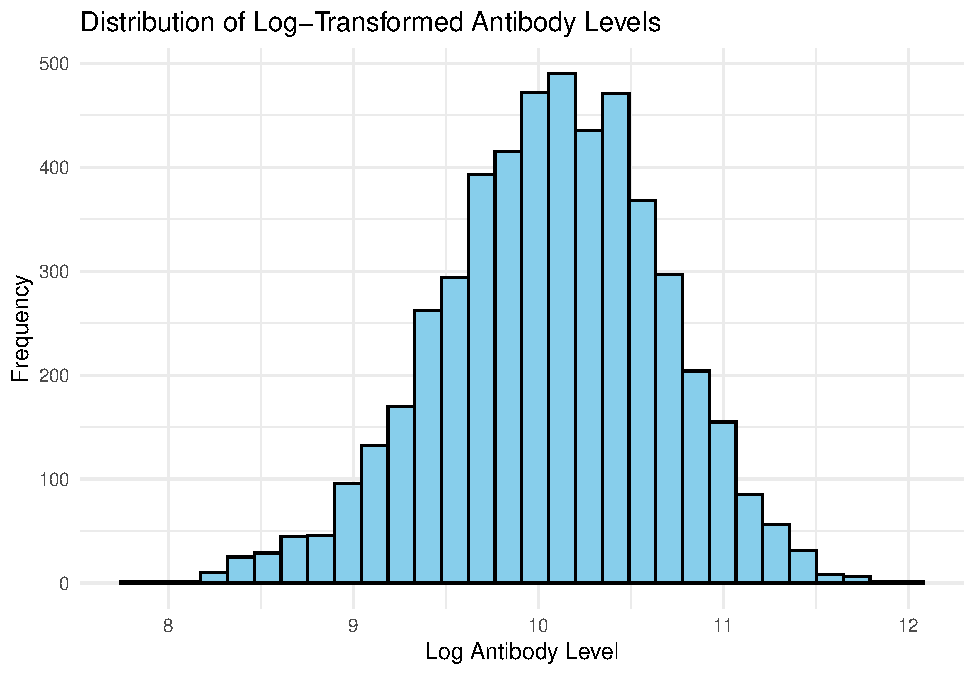
\includegraphics{p8106_midterm_project_files/figure-latex/unnamed-chunk-9-1.pdf}

\subsubsection{2.2 Boxplot of log
antibody}\label{boxplot-of-log-antibody}

\begin{Shaded}
\begin{Highlighting}[]
\CommentTok{\# Boxplot of log\_antibody by gender}
\NormalTok{p2 }\OtherTok{\textless{}{-}} \FunctionTok{ggplot}\NormalTok{(dat1, }\FunctionTok{aes}\NormalTok{(}\AttributeTok{x =}\NormalTok{ gender, }\AttributeTok{y =}\NormalTok{ log\_antibody, }\AttributeTok{fill =}\NormalTok{ gender)) }\SpecialCharTok{+}
  \FunctionTok{geom\_boxplot}\NormalTok{() }\SpecialCharTok{+}
  \FunctionTok{labs}\NormalTok{(}\AttributeTok{title =} \StringTok{"Antibody Levels by Gender"}\NormalTok{,}
       \AttributeTok{x =} \StringTok{"Gender"}\NormalTok{, }
       \AttributeTok{y =} \StringTok{"Log Antibody Level"}\NormalTok{) }\SpecialCharTok{+}
  \FunctionTok{theme\_minimal}\NormalTok{()}

\CommentTok{\# Boxplot of log\_antibody by race}
\NormalTok{p3 }\OtherTok{\textless{}{-}} \FunctionTok{ggplot}\NormalTok{(dat1, }\FunctionTok{aes}\NormalTok{(}\AttributeTok{x =}\NormalTok{ race, }\AttributeTok{y =}\NormalTok{ log\_antibody, }\AttributeTok{fill =}\NormalTok{ race)) }\SpecialCharTok{+}
  \FunctionTok{geom\_boxplot}\NormalTok{() }\SpecialCharTok{+}
  \FunctionTok{labs}\NormalTok{(}\AttributeTok{title =} \StringTok{"Antibody Levels by Race/Ethnicity"}\NormalTok{,}
       \AttributeTok{x =} \StringTok{"Race/Ethnicity"}\NormalTok{, }
       \AttributeTok{y =} \StringTok{"Log Antibody Level"}\NormalTok{) }\SpecialCharTok{+}
  \FunctionTok{theme\_minimal}\NormalTok{()}

\CommentTok{\# Boxplot of log\_antibody by smoking status}
\NormalTok{p4 }\OtherTok{\textless{}{-}} \FunctionTok{ggplot}\NormalTok{(dat1, }\FunctionTok{aes}\NormalTok{(}\AttributeTok{x =}\NormalTok{ smoking, }\AttributeTok{y =}\NormalTok{ log\_antibody, }\AttributeTok{fill =}\NormalTok{ smoking)) }\SpecialCharTok{+}
  \FunctionTok{geom\_boxplot}\NormalTok{() }\SpecialCharTok{+}
  \FunctionTok{labs}\NormalTok{(}\AttributeTok{title =} \StringTok{"Antibody Levels by Smoking Status"}\NormalTok{,}
       \AttributeTok{x =} \StringTok{"Smoking Status"}\NormalTok{, }
       \AttributeTok{y =} \StringTok{"Log Antibody Level"}\NormalTok{) }\SpecialCharTok{+}
  \FunctionTok{theme\_minimal}\NormalTok{()}

\CommentTok{\# Boxplot of log\_antibody by diabetes status}
\NormalTok{p5 }\OtherTok{\textless{}{-}} \FunctionTok{ggplot}\NormalTok{(dat1, }\FunctionTok{aes}\NormalTok{(}\AttributeTok{x =}\NormalTok{ diabetes, }\AttributeTok{y =}\NormalTok{ log\_antibody, }\AttributeTok{fill =}\NormalTok{ diabetes)) }\SpecialCharTok{+}
  \FunctionTok{geom\_boxplot}\NormalTok{() }\SpecialCharTok{+}
  \FunctionTok{labs}\NormalTok{(}\AttributeTok{title =} \StringTok{"Antibody Levels by Diabetes Status"}\NormalTok{,}
       \AttributeTok{x =} \StringTok{"Diabetes Status"}\NormalTok{, }
       \AttributeTok{y =} \StringTok{"Log Antibody Level"}\NormalTok{) }\SpecialCharTok{+}
  \FunctionTok{theme\_minimal}\NormalTok{()}
\end{Highlighting}
\end{Shaded}

\begin{Shaded}
\begin{Highlighting}[]
\NormalTok{p2}\SpecialCharTok{+}\NormalTok{p3}\SpecialCharTok{+}\NormalTok{p4}\SpecialCharTok{+}\NormalTok{p5}
\end{Highlighting}
\end{Shaded}

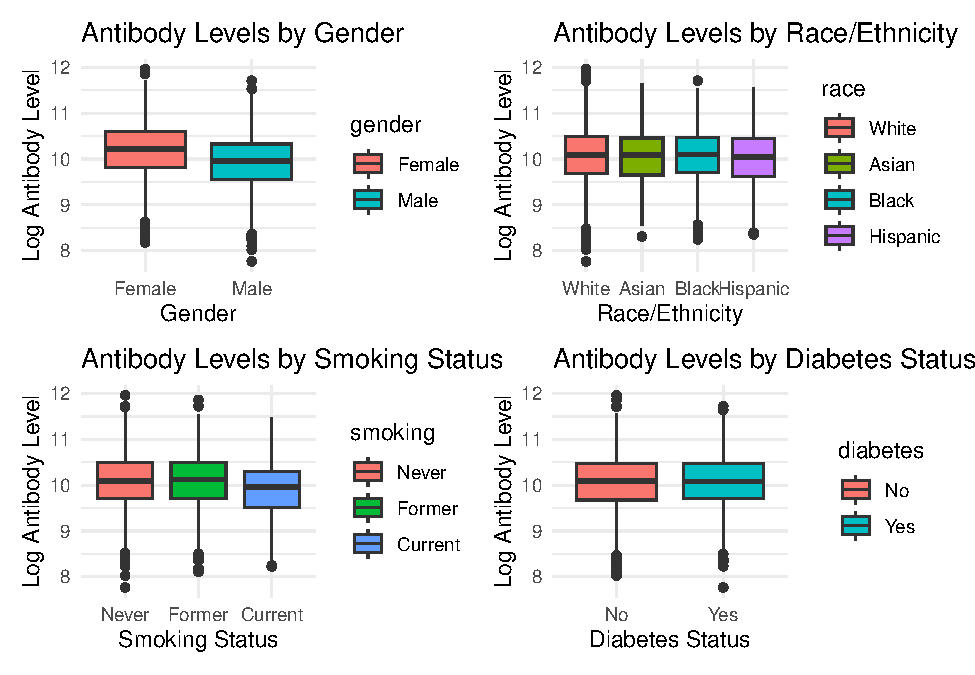
\includegraphics{p8106_midterm_project_files/figure-latex/unnamed-chunk-11-1.pdf}

\subsubsection{2.3 Correlation Plot}\label{correlation-plot}

\begin{Shaded}
\begin{Highlighting}[]
\CommentTok{\# Scatterplot matrix for continuous variables}
\NormalTok{continuous\_vars }\OtherTok{\textless{}{-}}\NormalTok{ dat1 }\SpecialCharTok{\%\textgreater{}\%} 
  \FunctionTok{select}\NormalTok{(age, height, weight, bmi, sbp, ldl, time, log\_antibody)}

\CommentTok{\# Calculate correlation matrix}
\NormalTok{correlation\_matrix }\OtherTok{\textless{}{-}} \FunctionTok{cor}\NormalTok{(continuous\_vars)}
\FunctionTok{corrplot}\NormalTok{(correlation\_matrix, }\AttributeTok{method =} \StringTok{"circle"}\NormalTok{, }\AttributeTok{type =} \StringTok{"upper"}\NormalTok{, }
         \AttributeTok{tl.col =} \StringTok{"black"}\NormalTok{, }\AttributeTok{tl.srt =} \DecValTok{45}\NormalTok{)}
\end{Highlighting}
\end{Shaded}

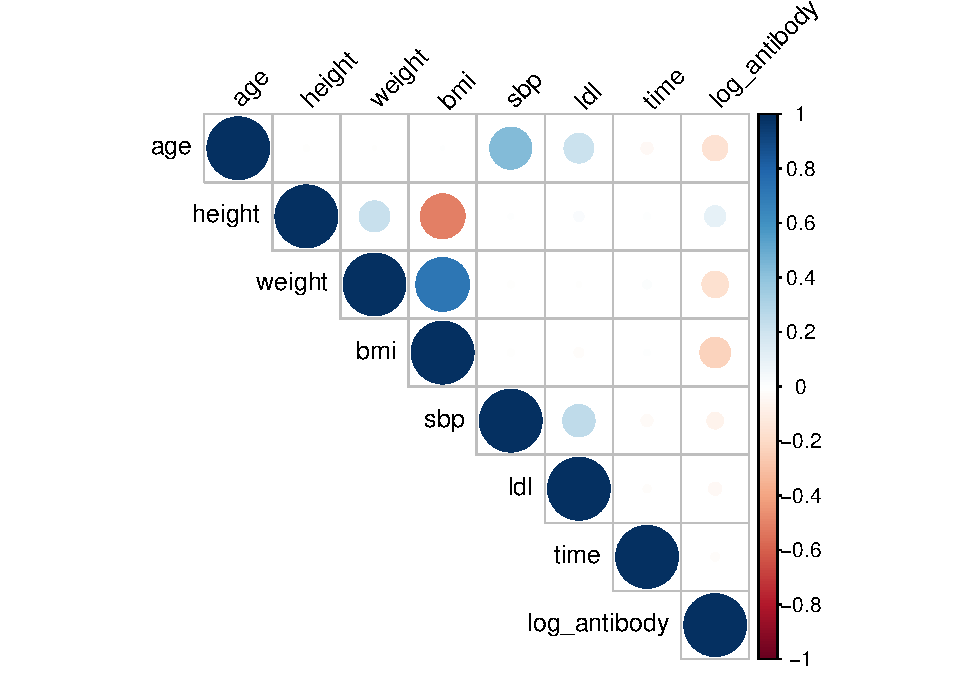
\includegraphics{p8106_midterm_project_files/figure-latex/unnamed-chunk-12-1.pdf}

\subsubsection{2.4 Scatterplots}\label{scatterplots}

\begin{Shaded}
\begin{Highlighting}[]
\CommentTok{\# Create scatterplots for continuous variables vs response}
\NormalTok{p6 }\OtherTok{\textless{}{-}} \FunctionTok{ggplot}\NormalTok{(dat1, }\FunctionTok{aes}\NormalTok{(}\AttributeTok{x =}\NormalTok{ age, }\AttributeTok{y =}\NormalTok{ log\_antibody)) }\SpecialCharTok{+}
  \FunctionTok{geom\_point}\NormalTok{(}\AttributeTok{alpha =} \FloatTok{0.5}\NormalTok{) }\SpecialCharTok{+}
  \FunctionTok{geom\_smooth}\NormalTok{(}\AttributeTok{method =} \StringTok{"loess"}\NormalTok{, }\AttributeTok{color =} \StringTok{"red"}\NormalTok{) }\SpecialCharTok{+}
  \FunctionTok{labs}\NormalTok{(}\AttributeTok{title =} \StringTok{"Age vs Log Antibody Level"}\NormalTok{, }
       \AttributeTok{x =} \StringTok{"Age (years)"}\NormalTok{, }\AttributeTok{y =} \StringTok{"Log Antibody Level"}\NormalTok{) }\SpecialCharTok{+}
  \FunctionTok{theme\_minimal}\NormalTok{()}

\NormalTok{p7 }\OtherTok{\textless{}{-}} \FunctionTok{ggplot}\NormalTok{(dat1, }\FunctionTok{aes}\NormalTok{(}\AttributeTok{x =}\NormalTok{ bmi, }\AttributeTok{y =}\NormalTok{ log\_antibody)) }\SpecialCharTok{+}
  \FunctionTok{geom\_point}\NormalTok{(}\AttributeTok{alpha =} \FloatTok{0.5}\NormalTok{) }\SpecialCharTok{+}
  \FunctionTok{geom\_smooth}\NormalTok{(}\AttributeTok{method =} \StringTok{"loess"}\NormalTok{, }\AttributeTok{color =} \StringTok{"red"}\NormalTok{) }\SpecialCharTok{+}
  \FunctionTok{labs}\NormalTok{(}\AttributeTok{title =} \StringTok{"BMI vs Log Antibody Level"}\NormalTok{, }
       \AttributeTok{x =} \StringTok{"BMI"}\NormalTok{, }\AttributeTok{y =} \StringTok{"Log Antibody Level"}\NormalTok{) }\SpecialCharTok{+}
  \FunctionTok{theme\_minimal}\NormalTok{()}

\NormalTok{p8 }\OtherTok{\textless{}{-}} \FunctionTok{ggplot}\NormalTok{(dat1, }\FunctionTok{aes}\NormalTok{(}\AttributeTok{x =}\NormalTok{ time, }\AttributeTok{y =}\NormalTok{ log\_antibody)) }\SpecialCharTok{+}
  \FunctionTok{geom\_point}\NormalTok{(}\AttributeTok{alpha =} \FloatTok{0.5}\NormalTok{) }\SpecialCharTok{+}
  \FunctionTok{geom\_smooth}\NormalTok{(}\AttributeTok{method =} \StringTok{"loess"}\NormalTok{, }\AttributeTok{color =} \StringTok{"red"}\NormalTok{) }\SpecialCharTok{+}
  \FunctionTok{labs}\NormalTok{(}\AttributeTok{title =} \StringTok{"Time Since Vaccination vs Log Antibody Level"}\NormalTok{, }
       \AttributeTok{x =} \StringTok{"Time (days)"}\NormalTok{, }\AttributeTok{y =} \StringTok{"Log Antibody Level"}\NormalTok{) }\SpecialCharTok{+}
  \FunctionTok{theme\_minimal}\NormalTok{()}
\end{Highlighting}
\end{Shaded}

\begin{Shaded}
\begin{Highlighting}[]
\NormalTok{p6}\SpecialCharTok{+}\NormalTok{p7}\SpecialCharTok{+}\NormalTok{p8}
\end{Highlighting}
\end{Shaded}

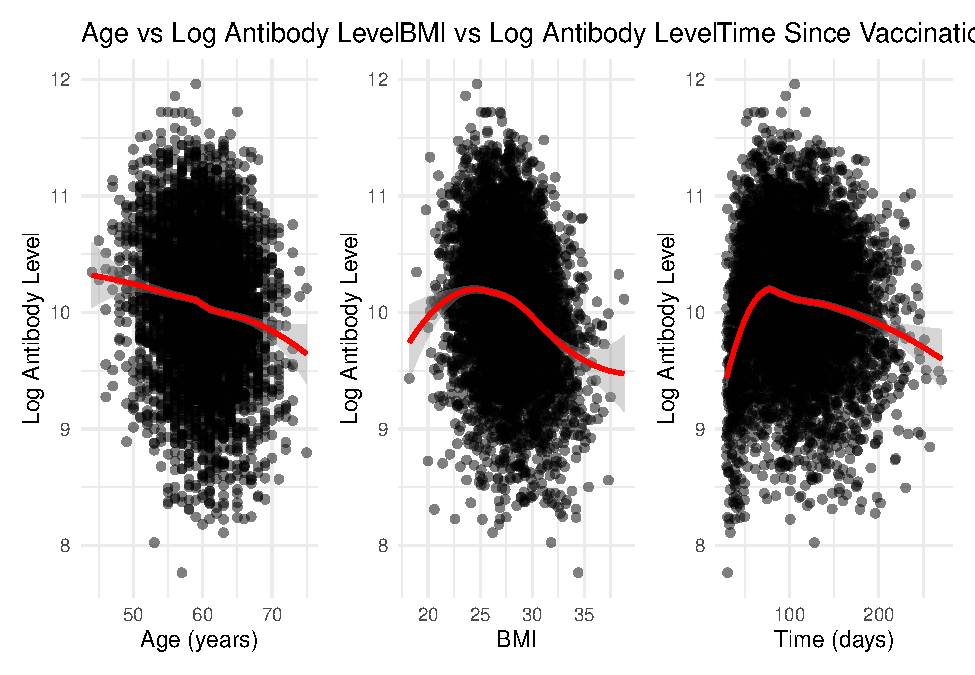
\includegraphics{p8106_midterm_project_files/figure-latex/unnamed-chunk-14-1.pdf}
There are some potential nonlinear trend between log\_antibody and bmi,
and between log\_antibody and time.

\subsection{3. Model Training with
Cross-validation}\label{model-training-with-cross-validation}

\subsubsection{3.1 Linear models}\label{linear-models}

\paragraph{3.1.1 Linear regression}\label{linear-regression}

\begin{Shaded}
\begin{Highlighting}[]
\NormalTok{model\_formula }\OtherTok{\textless{}{-}}\NormalTok{ log\_antibody }\SpecialCharTok{\textasciitilde{}}\NormalTok{ . }\SpecialCharTok{{-}}\NormalTok{ id}

\CommentTok{\# Set up cross{-}validation control}
\NormalTok{ctrl }\OtherTok{\textless{}{-}} \FunctionTok{trainControl}\NormalTok{(}\AttributeTok{method =} \StringTok{"cv"}\NormalTok{, }\AttributeTok{number =} \DecValTok{10}\NormalTok{)}

\CommentTok{\# 3.1 Linear Regression}
\FunctionTok{set.seed}\NormalTok{(}\DecValTok{123}\NormalTok{)}
\NormalTok{lm.fit }\OtherTok{\textless{}{-}} \FunctionTok{train}\NormalTok{(}
\NormalTok{  model\_formula,}
  \AttributeTok{data =}\NormalTok{ dat1,}
  \AttributeTok{method =} \StringTok{"lm"}\NormalTok{,}
  \AttributeTok{trControl =}\NormalTok{ ctrl}
\NormalTok{)}
\FunctionTok{summary}\NormalTok{(lm.fit}\SpecialCharTok{$}\NormalTok{finalModel)}
\end{Highlighting}
\end{Shaded}

\begin{verbatim}
## 
## Call:
## lm(formula = .outcome ~ ., data = dat)
## 
## Residuals:
##      Min       1Q   Median       3Q      Max 
## -2.14396 -0.35840  0.02944  0.37802  1.65090 
## 
## Coefficients:
##                   Estimate Std. Error t value Pr(>|t|)    
## (Intercept)     26.6751961  2.3149812  11.523  < 2e-16 ***
## age             -0.0205979  0.0019385 -10.626  < 2e-16 ***
## genderMale      -0.2974929  0.0155977 -19.073  < 2e-16 ***
## raceAsian       -0.0060422  0.0344613  -0.175   0.8608    
## raceBlack       -0.0075295  0.0196815  -0.383   0.7021    
## raceHispanic    -0.0417571  0.0273309  -1.528   0.1266    
## smokingFormer    0.0219907  0.0173992   1.264   0.2063    
## smokingCurrent  -0.1934834  0.0269576  -7.177 8.15e-13 ***
## height          -0.0821381  0.0135622  -6.056 1.49e-09 ***
## weight           0.0859034  0.0143481   5.987 2.29e-09 ***
## bmi             -0.2977935  0.0412612  -7.217 6.10e-13 ***
## diabetesYes      0.0112795  0.0215643   0.523   0.6010    
## hypertensionYes -0.0179106  0.0260931  -0.686   0.4925    
## sbp              0.0015181  0.0017049   0.890   0.3733    
## ldl             -0.0001645  0.0004028  -0.409   0.6829    
## time            -0.0003011  0.0001795  -1.677   0.0936 .  
## ---
## Signif. codes:  0 '***' 0.001 '**' 0.01 '*' 0.05 '.' 0.1 ' ' 1
## 
## Residual standard error: 0.5503 on 4984 degrees of freedom
## Multiple R-squared:  0.1513, Adjusted R-squared:  0.1488 
## F-statistic: 59.25 on 15 and 4984 DF,  p-value: < 2.2e-16
\end{verbatim}

\paragraph{3.1.2 Ridge Regression}\label{ridge-regression}

\begin{Shaded}
\begin{Highlighting}[]
\FunctionTok{set.seed}\NormalTok{(}\DecValTok{123}\NormalTok{)}
\NormalTok{ridge.fit }\OtherTok{\textless{}{-}} \FunctionTok{train}\NormalTok{(}
\NormalTok{  model\_formula,}
  \AttributeTok{data =}\NormalTok{ dat1,}
  \AttributeTok{method =} \StringTok{"glmnet"}\NormalTok{,}
  \AttributeTok{tuneGrid =} \FunctionTok{expand.grid}\NormalTok{(}\AttributeTok{alpha =} \DecValTok{0}\NormalTok{,}
                         \AttributeTok{lambda =} \FunctionTok{exp}\NormalTok{(}\FunctionTok{seq}\NormalTok{(}\DecValTok{6}\NormalTok{, }\SpecialCharTok{{-}}\DecValTok{6}\NormalTok{, }\AttributeTok{length =} \DecValTok{100}\NormalTok{))),}
  \AttributeTok{trControl =}\NormalTok{ ctrl}
\NormalTok{)}

\FunctionTok{coef}\NormalTok{(ridge.fit}\SpecialCharTok{$}\NormalTok{finalModel, }\AttributeTok{s =}\NormalTok{ ridge.fit}\SpecialCharTok{$}\NormalTok{bestTune}\SpecialCharTok{$}\NormalTok{lambda)}
\end{Highlighting}
\end{Shaded}

\begin{verbatim}
## 16 x 1 sparse Matrix of class "dgCMatrix"
##                            s1
## (Intercept)     12.7384560516
## age             -0.0197679168
## genderMale      -0.2880871615
## raceAsian       -0.0038318346
## raceBlack       -0.0066654722
## raceHispanic    -0.0417690245
## smokingFormer    0.0242172365
## smokingCurrent  -0.1847225211
## height          -0.0001949552
## weight          -0.0009185524
## bmi             -0.0473178893
## diabetesYes      0.0113069924
## hypertensionYes -0.0166641972
## sbp              0.0010847735
## ldl             -0.0001614795
## time            -0.0002807285
\end{verbatim}

\begin{Shaded}
\begin{Highlighting}[]
\FunctionTok{print}\NormalTok{(ridge.fit}\SpecialCharTok{$}\NormalTok{bestTune)}
\end{Highlighting}
\end{Shaded}

\begin{verbatim}
##    alpha    lambda
## 15     0 0.0135275
\end{verbatim}

\begin{Shaded}
\begin{Highlighting}[]
\FunctionTok{plot}\NormalTok{(ridge.fit, }\AttributeTok{xTrans =}\NormalTok{ log)}
\end{Highlighting}
\end{Shaded}

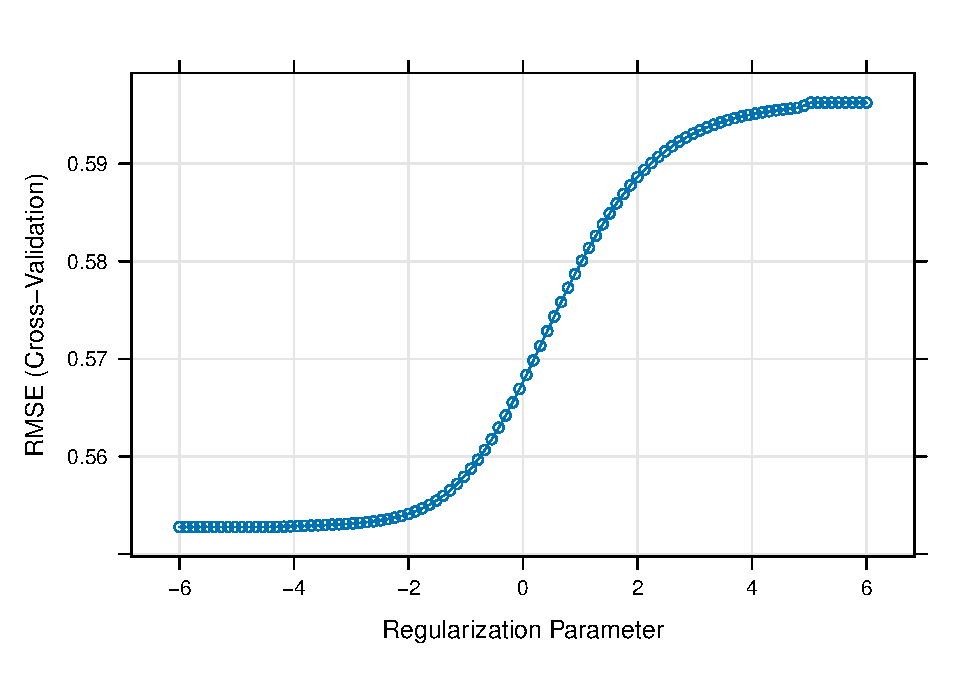
\includegraphics{p8106_midterm_project_files/figure-latex/unnamed-chunk-16-1.pdf}

\paragraph{3.1.3 Lasso Regression}\label{lasso-regression}

\begin{Shaded}
\begin{Highlighting}[]
\FunctionTok{set.seed}\NormalTok{(}\DecValTok{123}\NormalTok{)}
\NormalTok{lasso.fit }\OtherTok{\textless{}{-}} \FunctionTok{train}\NormalTok{(}
\NormalTok{  model\_formula,}
  \AttributeTok{data =}\NormalTok{ dat1, }
  \AttributeTok{method =} \StringTok{"glmnet"}\NormalTok{,}
  \AttributeTok{tuneGrid =} \FunctionTok{expand.grid}\NormalTok{(}\AttributeTok{alpha =} \DecValTok{1}\NormalTok{,}
                         \AttributeTok{lambda =} \FunctionTok{exp}\NormalTok{(}\FunctionTok{seq}\NormalTok{(}\DecValTok{6}\NormalTok{, }\SpecialCharTok{{-}}\DecValTok{6}\NormalTok{, }\AttributeTok{length =} \DecValTok{100}\NormalTok{))),}
  \AttributeTok{trControl =}\NormalTok{ ctrl}
\NormalTok{)}

\FunctionTok{coef}\NormalTok{(lasso.fit}\SpecialCharTok{$}\NormalTok{finalModel, lasso.fit}\SpecialCharTok{$}\NormalTok{bestTune}\SpecialCharTok{$}\NormalTok{lambda)}
\end{Highlighting}
\end{Shaded}

\begin{verbatim}
## 16 x 1 sparse Matrix of class "dgCMatrix"
##                            s1
## (Intercept)      1.272648e+01
## age             -1.915006e-02
## genderMale      -2.859715e-01
## raceAsian        .           
## raceBlack        .           
## raceHispanic    -2.472809e-02
## smokingFormer    1.593301e-02
## smokingCurrent  -1.770968e-01
## height           .           
## weight          -1.029699e-04
## bmi             -4.801089e-02
## diabetesYes      4.273525e-05
## hypertensionYes  .           
## sbp              .           
## ldl              .           
## time            -1.848766e-04
\end{verbatim}

\begin{Shaded}
\begin{Highlighting}[]
\FunctionTok{print}\NormalTok{(lasso.fit}\SpecialCharTok{$}\NormalTok{bestTune)}
\end{Highlighting}
\end{Shaded}

\begin{verbatim}
##   alpha      lambda
## 6     1 0.004544037
\end{verbatim}

\begin{Shaded}
\begin{Highlighting}[]
\FunctionTok{plot}\NormalTok{(lasso.fit, }\AttributeTok{xTrans =}\NormalTok{ log)}
\end{Highlighting}
\end{Shaded}

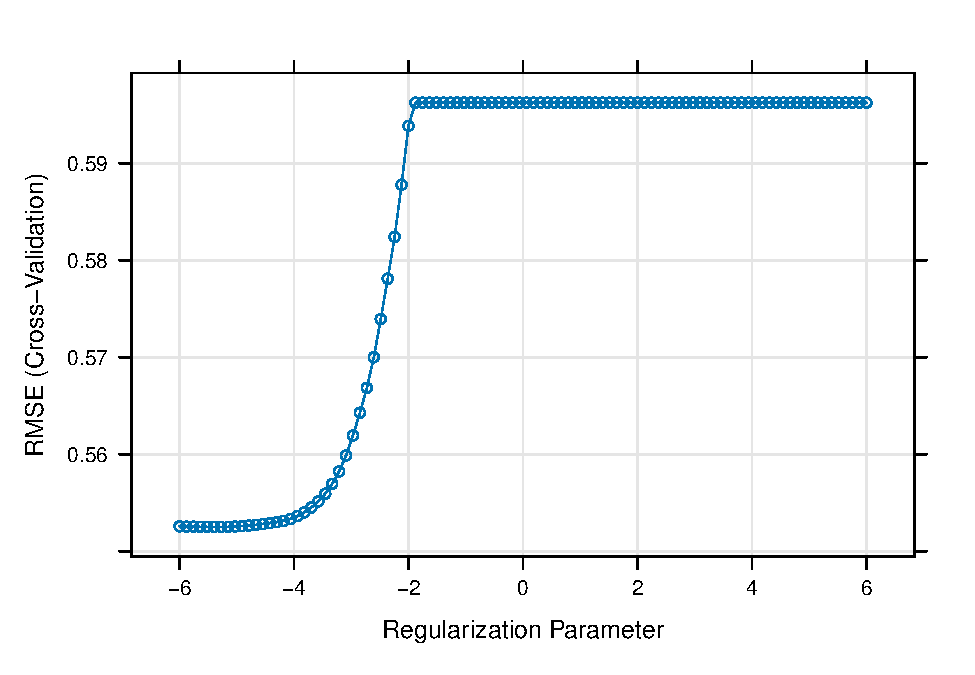
\includegraphics{p8106_midterm_project_files/figure-latex/unnamed-chunk-17-1.pdf}

\paragraph{3.1.4 Elastic Net Regression}\label{elastic-net-regression}

\begin{Shaded}
\begin{Highlighting}[]
\FunctionTok{set.seed}\NormalTok{(}\DecValTok{123}\NormalTok{)}
\NormalTok{enet.fit }\OtherTok{\textless{}{-}} \FunctionTok{train}\NormalTok{(}
\NormalTok{  model\_formula,}
  \AttributeTok{data =}\NormalTok{ dat1,}
  \AttributeTok{method =} \StringTok{"glmnet"}\NormalTok{,}
  \AttributeTok{tuneGrid =} \FunctionTok{expand.grid}\NormalTok{(}\AttributeTok{alpha =} \FunctionTok{seq}\NormalTok{(}\DecValTok{0}\NormalTok{, }\DecValTok{1}\NormalTok{, }\AttributeTok{length =} \DecValTok{21}\NormalTok{),}
                         \AttributeTok{lambda =} \FunctionTok{exp}\NormalTok{(}\FunctionTok{seq}\NormalTok{(}\DecValTok{6}\NormalTok{, }\SpecialCharTok{{-}}\DecValTok{6}\NormalTok{, }\AttributeTok{length =} \DecValTok{100}\NormalTok{))),}
  \AttributeTok{trControl =}\NormalTok{ ctrl}
\NormalTok{)}
\FunctionTok{summary}\NormalTok{(enet.fit)}
\end{Highlighting}
\end{Shaded}

\begin{verbatim}
##             Length Class      Mode     
## a0           100   -none-     numeric  
## beta        1500   dgCMatrix  S4       
## df           100   -none-     numeric  
## dim            2   -none-     numeric  
## lambda       100   -none-     numeric  
## dev.ratio    100   -none-     numeric  
## nulldev        1   -none-     numeric  
## npasses        1   -none-     numeric  
## jerr           1   -none-     numeric  
## offset         1   -none-     logical  
## call           5   -none-     call     
## nobs           1   -none-     numeric  
## lambdaOpt      1   -none-     numeric  
## xNames        15   -none-     character
## problemType    1   -none-     character
## tuneValue      2   data.frame list     
## obsLevels      1   -none-     logical  
## param          0   -none-     list
\end{verbatim}

\begin{Shaded}
\begin{Highlighting}[]
\FunctionTok{print}\NormalTok{(enet.fit}\SpecialCharTok{$}\NormalTok{bestTune)}
\end{Highlighting}
\end{Shaded}

\begin{verbatim}
##     alpha      lambda
## 101  0.05 0.002478752
\end{verbatim}

\begin{Shaded}
\begin{Highlighting}[]
\CommentTok{\# Plot elastic net results with different colors for each alpha}
\NormalTok{myCol }\OtherTok{\textless{}{-}} \FunctionTok{rainbow}\NormalTok{(}\DecValTok{25}\NormalTok{)}
\NormalTok{myPar }\OtherTok{\textless{}{-}} \FunctionTok{list}\NormalTok{(}\AttributeTok{superpose.symbol =} \FunctionTok{list}\NormalTok{(}\AttributeTok{col =}\NormalTok{ myCol),}
              \AttributeTok{superpose.line =} \FunctionTok{list}\NormalTok{(}\AttributeTok{col =}\NormalTok{ myCol))}
\FunctionTok{plot}\NormalTok{(enet.fit, }\AttributeTok{par.settings =}\NormalTok{ myPar, }\AttributeTok{xTrans =}\NormalTok{ log)}
\end{Highlighting}
\end{Shaded}

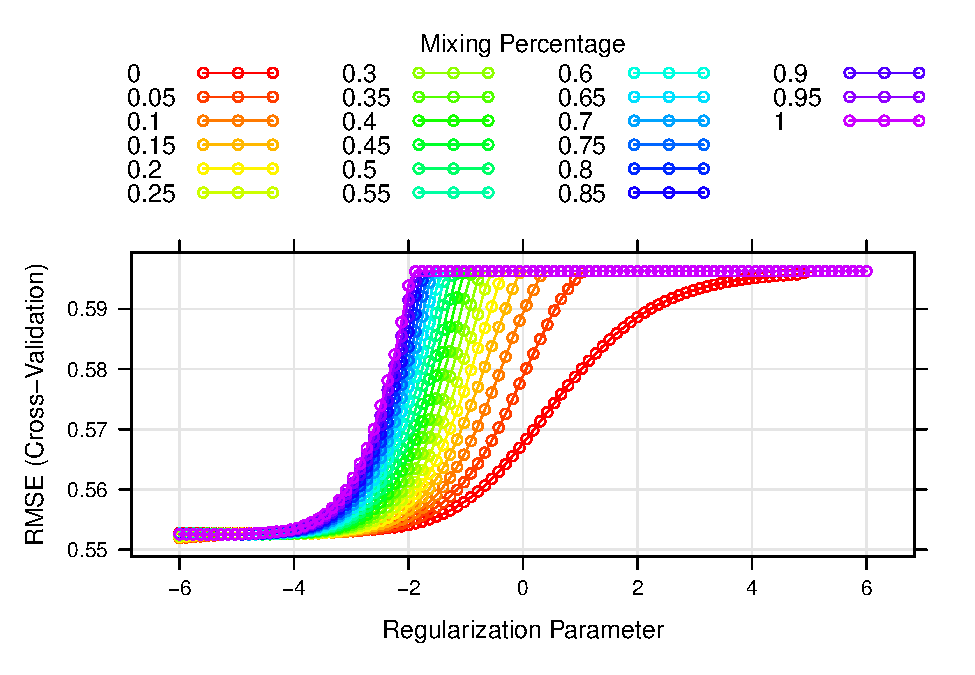
\includegraphics{p8106_midterm_project_files/figure-latex/unnamed-chunk-19-1.pdf}

\begin{Shaded}
\begin{Highlighting}[]
\CommentTok{\# Show coefficients of the final Elastic Net model}
\NormalTok{coef\_enet }\OtherTok{\textless{}{-}} \FunctionTok{coef}\NormalTok{(enet.fit}\SpecialCharTok{$}\NormalTok{finalModel, enet.fit}\SpecialCharTok{$}\NormalTok{bestTune}\SpecialCharTok{$}\NormalTok{lambda)}
\FunctionTok{print}\NormalTok{(coef\_enet)}
\end{Highlighting}
\end{Shaded}

\begin{verbatim}
## 16 x 1 sparse Matrix of class "dgCMatrix"
##                            s1
## (Intercept)     16.0225822334
## age             -0.0202906145
## genderMale      -0.2942760076
## raceAsian       -0.0036856007
## raceBlack       -0.0066593257
## raceHispanic    -0.0417893824
## smokingFormer    0.0235504017
## smokingCurrent  -0.1891969582
## height          -0.0193618230
## weight           0.0193847860
## bmi             -0.1063133265
## diabetesYes      0.0111516911
## hypertensionYes -0.0167677112
## sbp              0.0012484795
## ldl             -0.0001495619
## time            -0.0002879691
\end{verbatim}

\begin{Shaded}
\begin{Highlighting}[]
\NormalTok{coef\_enet }\OtherTok{\textless{}{-}} \FunctionTok{coef}\NormalTok{(enet.fit}\SpecialCharTok{$}\NormalTok{finalModel, enet.fit}\SpecialCharTok{$}\NormalTok{bestTune}\SpecialCharTok{$}\NormalTok{lambda)}
\FunctionTok{print}\NormalTok{(coef\_enet)}
\end{Highlighting}
\end{Shaded}

\begin{verbatim}
## 16 x 1 sparse Matrix of class "dgCMatrix"
##                            s1
## (Intercept)     16.0225822334
## age             -0.0202906145
## genderMale      -0.2942760076
## raceAsian       -0.0036856007
## raceBlack       -0.0066593257
## raceHispanic    -0.0417893824
## smokingFormer    0.0235504017
## smokingCurrent  -0.1891969582
## height          -0.0193618230
## weight           0.0193847860
## bmi             -0.1063133265
## diabetesYes      0.0111516911
## hypertensionYes -0.0167677112
## sbp              0.0012484795
## ldl             -0.0001495619
## time            -0.0002879691
\end{verbatim}

\paragraph{3.1.5 Model Comparison
(resampling)}\label{model-comparison-resampling}

\begin{Shaded}
\begin{Highlighting}[]
\NormalTok{resamp }\OtherTok{\textless{}{-}} \FunctionTok{resamples}\NormalTok{(}\FunctionTok{list}\NormalTok{(}
  \AttributeTok{Linear\_Regression =}\NormalTok{ lm.fit,}
  \AttributeTok{Ridge =}\NormalTok{ ridge.fit, }
  \AttributeTok{Lasso =}\NormalTok{ lasso.fit,}
  \AttributeTok{Elastic\_Net =}\NormalTok{ enet.fit}
\NormalTok{))}
\FunctionTok{summary}\NormalTok{(resamp)}
\end{Highlighting}
\end{Shaded}

\begin{verbatim}
## 
## Call:
## summary.resamples(object = resamp)
## 
## Models: Linear_Regression, Ridge, Lasso, Elastic_Net 
## Number of resamples: 10 
## 
## MAE 
##                        Min.   1st Qu.    Median      Mean   3rd Qu.      Max.
## Linear_Regression 0.4261808 0.4320149 0.4340128 0.4390390 0.4425761 0.4726409
## Ridge             0.4281731 0.4334230 0.4362590 0.4405051 0.4454071 0.4720434
## Lasso             0.4276920 0.4330647 0.4364914 0.4403860 0.4449243 0.4721327
## Elastic_Net       0.4274328 0.4330542 0.4354391 0.4399269 0.4448176 0.4720702
##                   NA's
## Linear_Regression    0
## Ridge                0
## Lasso                0
## Elastic_Net          0
## 
## RMSE 
##                        Min.   1st Qu.    Median      Mean   3rd Qu.      Max.
## Linear_Regression 0.5325907 0.5394231 0.5513718 0.5507854 0.5564032 0.5835238
## Ridge             0.5363406 0.5426274 0.5535668 0.5527796 0.5570390 0.5837848
## Lasso             0.5362188 0.5422580 0.5529754 0.5525153 0.5572793 0.5834368
## Elastic_Net       0.5354741 0.5414764 0.5531955 0.5519547 0.5560081 0.5834749
##                   NA's
## Linear_Regression    0
## Ridge                0
## Lasso                0
## Elastic_Net          0
## 
## Rsquared 
##                         Min.   1st Qu.    Median      Mean   3rd Qu.      Max.
## Linear_Regression 0.10033968 0.1319832 0.1534930 0.1479018 0.1622355 0.1906302
## Ridge             0.09354935 0.1329969 0.1421825 0.1418538 0.1502030 0.1878098
## Lasso             0.09475560 0.1342489 0.1433703 0.1428172 0.1503016 0.1912475
## Elastic_Net       0.09585259 0.1339416 0.1458955 0.1443698 0.1542137 0.1902642
##                   NA's
## Linear_Regression    0
## Ridge                0
## Lasso                0
## Elastic_Net          0
\end{verbatim}

\begin{Shaded}
\begin{Highlighting}[]
\FunctionTok{parallelplot}\NormalTok{(resamp, }\AttributeTok{metric =} \StringTok{"RMSE"}\NormalTok{)}
\end{Highlighting}
\end{Shaded}

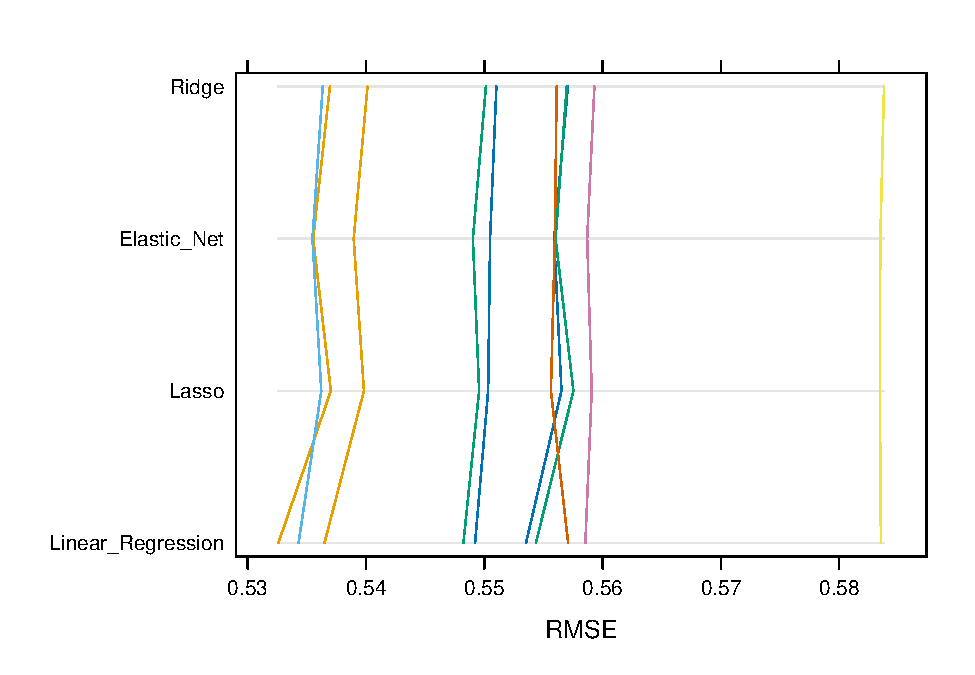
\includegraphics{p8106_midterm_project_files/figure-latex/unnamed-chunk-22-1.pdf}

\begin{Shaded}
\begin{Highlighting}[]
\FunctionTok{bwplot}\NormalTok{(resamp, }\AttributeTok{metric =} \StringTok{"RMSE"}\NormalTok{)}
\end{Highlighting}
\end{Shaded}

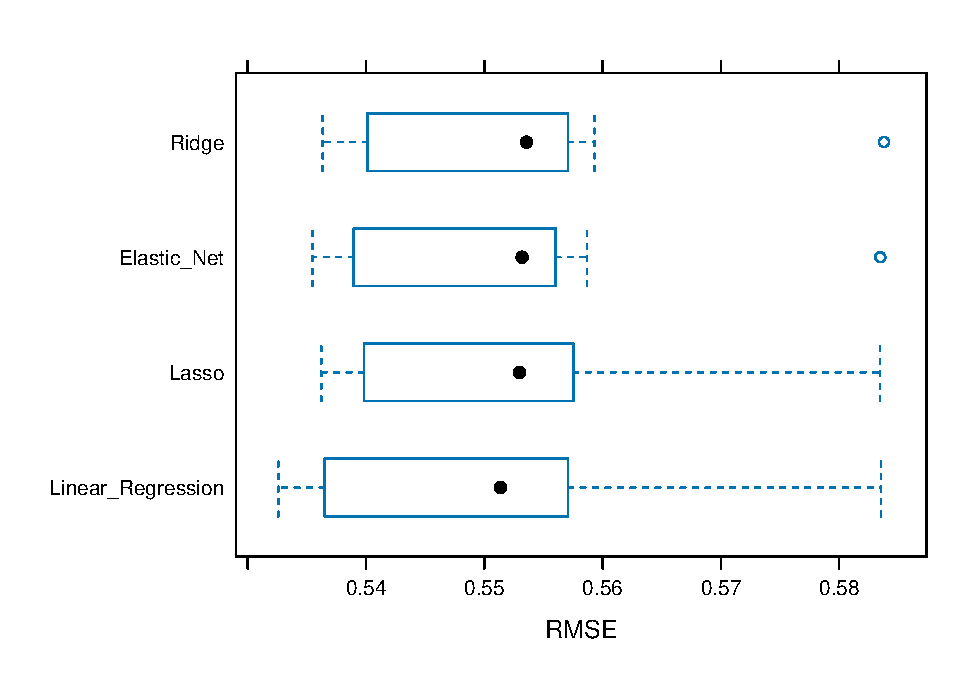
\includegraphics{p8106_midterm_project_files/figure-latex/unnamed-chunk-22-2.pdf}
The RMSE from resampling looks similar to each other.

\paragraph{3.1.6 Test Set Performance}\label{test-set-performance}

\begin{Shaded}
\begin{Highlighting}[]
\CommentTok{\# Function to calculate RMSE}
\NormalTok{rmse }\OtherTok{\textless{}{-}} \ControlFlowTok{function}\NormalTok{(actual, predicted) \{}
  \FunctionTok{sqrt}\NormalTok{(}\FunctionTok{mean}\NormalTok{((actual }\SpecialCharTok{{-}}\NormalTok{ predicted)}\SpecialCharTok{\^{}}\DecValTok{2}\NormalTok{))}
\NormalTok{\}}
\end{Highlighting}
\end{Shaded}

\begin{Shaded}
\begin{Highlighting}[]
\CommentTok{\# Make predictions using each model}
\NormalTok{lm.pred }\OtherTok{\textless{}{-}} \FunctionTok{predict}\NormalTok{(lm.fit, }\AttributeTok{newdata =}\NormalTok{ dat2)}
\NormalTok{ridge.pred }\OtherTok{\textless{}{-}} \FunctionTok{predict}\NormalTok{(ridge.fit, }\AttributeTok{newdata =}\NormalTok{ dat2)}
\NormalTok{lasso.pred }\OtherTok{\textless{}{-}} \FunctionTok{predict}\NormalTok{(lasso.fit, }\AttributeTok{newdata =}\NormalTok{ dat2)}
\NormalTok{enet.pred }\OtherTok{\textless{}{-}} \FunctionTok{predict}\NormalTok{(enet.fit, }\AttributeTok{newdata =}\NormalTok{ dat2)}
\end{Highlighting}
\end{Shaded}

\begin{Shaded}
\begin{Highlighting}[]
\CommentTok{\# Calculate test MSE for each model}
\NormalTok{lm.test.error }\OtherTok{\textless{}{-}} \FunctionTok{mean}\NormalTok{((lm.pred }\SpecialCharTok{{-}}\NormalTok{ dat2[,}\StringTok{"log\_antibody"}\NormalTok{])}\SpecialCharTok{\^{}}\DecValTok{2}\NormalTok{)}
\NormalTok{ridge.test.error }\OtherTok{\textless{}{-}} \FunctionTok{mean}\NormalTok{((ridge.pred }\SpecialCharTok{{-}}\NormalTok{ dat2[,}\StringTok{"log\_antibody"}\NormalTok{])}\SpecialCharTok{\^{}}\DecValTok{2}\NormalTok{)}
\NormalTok{lasso.test.error }\OtherTok{\textless{}{-}} \FunctionTok{mean}\NormalTok{((lasso.pred }\SpecialCharTok{{-}}\NormalTok{ dat2[,}\StringTok{"log\_antibody"}\NormalTok{])}\SpecialCharTok{\^{}}\DecValTok{2}\NormalTok{)}
\NormalTok{enet.test.error }\OtherTok{\textless{}{-}} \FunctionTok{mean}\NormalTok{((enet.pred }\SpecialCharTok{{-}}\NormalTok{ dat2[,}\StringTok{"log\_antibody"}\NormalTok{])}\SpecialCharTok{\^{}}\DecValTok{2}\NormalTok{)}
\end{Highlighting}
\end{Shaded}

\begin{Shaded}
\begin{Highlighting}[]
\NormalTok{test\_performance }\OtherTok{\textless{}{-}} \FunctionTok{data.frame}\NormalTok{(}
  \AttributeTok{Model =} \FunctionTok{c}\NormalTok{(}\StringTok{"Linear Regression"}\NormalTok{, }\StringTok{"Ridge Regression"}\NormalTok{, }\StringTok{"Lasso Regression"}\NormalTok{, }
            \StringTok{"Elastic Net Regression"}\NormalTok{),}
  \AttributeTok{Test\_ERROR =} \FunctionTok{c}\NormalTok{(lm.test.error, ridge.test.error, lasso.test.error, }
\NormalTok{                enet.test.error)}
\NormalTok{)}
\FunctionTok{print}\NormalTok{(test\_performance)}
\end{Highlighting}
\end{Shaded}

\begin{verbatim}
##                    Model Test_ERROR
## 1      Linear Regression  0.3229854
## 2       Ridge Regression  0.3258077
## 3       Lasso Regression  0.3288173
## 4 Elastic Net Regression  0.3247256
\end{verbatim}

They are very similar to each other. We probably want to choose the
Lasso model as it is the simplest model among those four models.

\subsubsection{3.2 Non-linear Models}\label{non-linear-models}

\paragraph{3.2.1 Smoothing Spline}\label{smoothing-spline}

We use scatterplot to explore the relationship between the log antibody
level and other variables. Time and bmi tend shows potentially nonlinear
trend.

\begin{Shaded}
\begin{Highlighting}[]
\NormalTok{x }\OtherTok{=} \FunctionTok{model.matrix}\NormalTok{(log\_antibody }\SpecialCharTok{\textasciitilde{}}\NormalTok{ . }\SpecialCharTok{{-}}\NormalTok{ id, }\AttributeTok{data =}\NormalTok{ dat1)[, }\SpecialCharTok{{-}}\DecValTok{1}\NormalTok{]}
\NormalTok{y }\OtherTok{=}\NormalTok{ dat1[,}\StringTok{"log\_antibody"}\NormalTok{]}
\NormalTok{x\_test }\OtherTok{=} \FunctionTok{model.matrix}\NormalTok{(log\_antibody }\SpecialCharTok{\textasciitilde{}}\NormalTok{ . }\SpecialCharTok{{-}}\NormalTok{ id, }\AttributeTok{data =}\NormalTok{ dat2)[, }\SpecialCharTok{{-}}\DecValTok{1}\NormalTok{]}
\NormalTok{y\_test }\OtherTok{=}\NormalTok{ dat2[,}\StringTok{"log\_antibody"}\NormalTok{]}
\end{Highlighting}
\end{Shaded}

\begin{Shaded}
\begin{Highlighting}[]
\CommentTok{\# choose the best df}
\NormalTok{fit.ss }\OtherTok{=} \FunctionTok{smooth.spline}\NormalTok{(dat1}\SpecialCharTok{$}\NormalTok{bmi, dat1}\SpecialCharTok{$}\NormalTok{log\_antibody)}
\NormalTok{fit.ss}\SpecialCharTok{$}\NormalTok{df}
\end{Highlighting}
\end{Shaded}

\begin{verbatim}
## [1] 5.769535
\end{verbatim}

\begin{Shaded}
\begin{Highlighting}[]
\FunctionTok{print}\NormalTok{(fit.ss)}
\end{Highlighting}
\end{Shaded}

\begin{verbatim}
## Call:
## smooth.spline(x = dat1$bmi, y = dat1$log_antibody)
## 
## Smoothing Parameter  spar= 0.8460071  lambda= 0.05288648 (13 iterations)
## Equivalent Degrees of Freedom (Df): 5.769535
## Penalized Criterion (RSS): 61.11728
## GCV: 0.3330358
\end{verbatim}

\begin{Shaded}
\begin{Highlighting}[]
\CommentTok{\# plot optimal fit}
\NormalTok{bmi.grid }\OtherTok{=} \FunctionTok{seq}\NormalTok{(}\AttributeTok{from =} \FloatTok{17.5}\NormalTok{, }\AttributeTok{to =} \DecValTok{40}\NormalTok{, }\AttributeTok{by =} \DecValTok{1}\NormalTok{)}

\NormalTok{pred.ss }\OtherTok{=} \FunctionTok{predict}\NormalTok{(fit.ss, }\AttributeTok{x =}\NormalTok{ bmi.grid)}
\NormalTok{pred.ss.df }\OtherTok{=} \FunctionTok{data.frame}\NormalTok{(}\AttributeTok{pred =}\NormalTok{ pred.ss}\SpecialCharTok{$}\NormalTok{y, }\AttributeTok{bmi =}\NormalTok{ bmi.grid)}


\NormalTok{p }\OtherTok{=} \FunctionTok{ggplot}\NormalTok{(dat1, }\FunctionTok{aes}\NormalTok{(}\AttributeTok{x =}\NormalTok{ bmi, }\AttributeTok{y =}\NormalTok{ log\_antibody)) }\SpecialCharTok{+}
  \FunctionTok{geom\_point}\NormalTok{(}\AttributeTok{color =} \FunctionTok{rgb}\NormalTok{(.}\DecValTok{2}\NormalTok{, .}\DecValTok{4}\NormalTok{, .}\DecValTok{2}\NormalTok{, .}\DecValTok{5}\NormalTok{), }\AttributeTok{size =} \DecValTok{1}\NormalTok{) }\SpecialCharTok{+} \FunctionTok{theme\_bw}\NormalTok{()}

\NormalTok{p }\SpecialCharTok{+}
\FunctionTok{geom\_line}\NormalTok{(}\FunctionTok{aes}\NormalTok{(}\AttributeTok{x =}\NormalTok{ bmi, }\AttributeTok{y =}\NormalTok{ pred), }\AttributeTok{data =}\NormalTok{ pred.ss.df,}
\AttributeTok{color =} \FunctionTok{rgb}\NormalTok{(.}\DecValTok{8}\NormalTok{, .}\DecValTok{1}\NormalTok{, .}\DecValTok{1}\NormalTok{, }\DecValTok{1}\NormalTok{)) }\SpecialCharTok{+} \FunctionTok{theme\_bw}\NormalTok{()}
\end{Highlighting}
\end{Shaded}

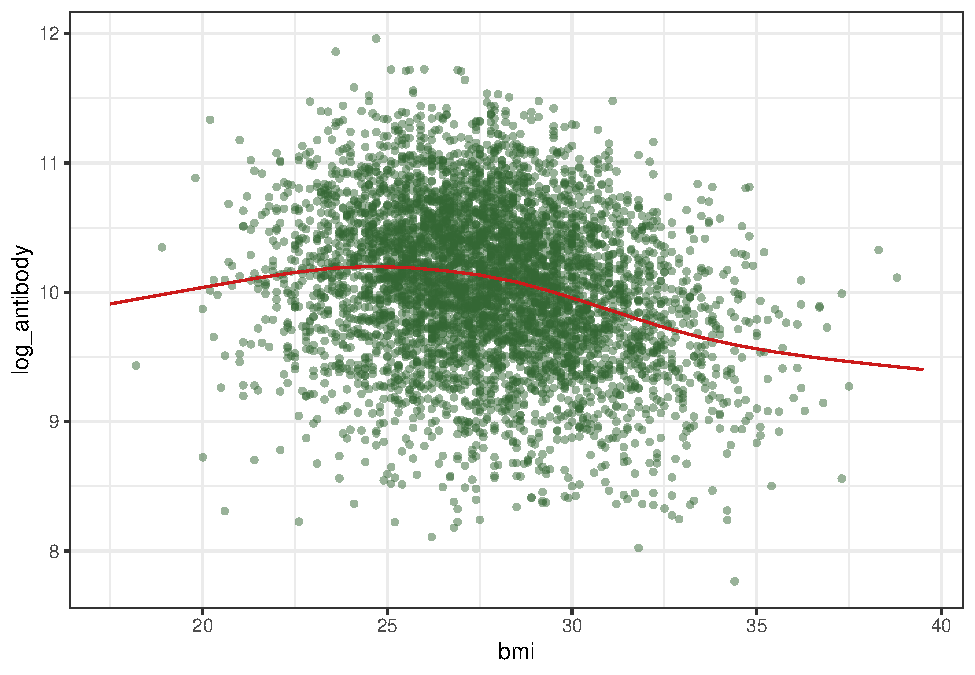
\includegraphics{p8106_midterm_project_files/figure-latex/unnamed-chunk-29-1.pdf}

\paragraph{3.2.2 Multivariate Adaptive Regression Splines
(MARS)}\label{multivariate-adaptive-regression-splines-mars}

\begin{Shaded}
\begin{Highlighting}[]
\FunctionTok{set.seed}\NormalTok{(}\DecValTok{2}\NormalTok{)}
\NormalTok{ctrl1 }\OtherTok{=} \FunctionTok{trainControl}\NormalTok{(}\AttributeTok{method =} \StringTok{"cv"}\NormalTok{, }\AttributeTok{number =} \DecValTok{10}\NormalTok{)}
\NormalTok{mars\_grid }\OtherTok{=} \FunctionTok{expand.grid}\NormalTok{(}\AttributeTok{degree =} \DecValTok{1}\SpecialCharTok{:}\DecValTok{3}\NormalTok{, }\AttributeTok{nprune =} \DecValTok{2}\SpecialCharTok{:}\DecValTok{20}\NormalTok{)}
\NormalTok{mars.fit }\OtherTok{=} \FunctionTok{train}\NormalTok{(x, y, }\AttributeTok{method =} \StringTok{"earth"}\NormalTok{, }\AttributeTok{tuneGrid =}\NormalTok{ mars\_grid,}
\AttributeTok{trControl =}\NormalTok{ ctrl1)}
\FunctionTok{ggplot}\NormalTok{(mars.fit)}
\end{Highlighting}
\end{Shaded}

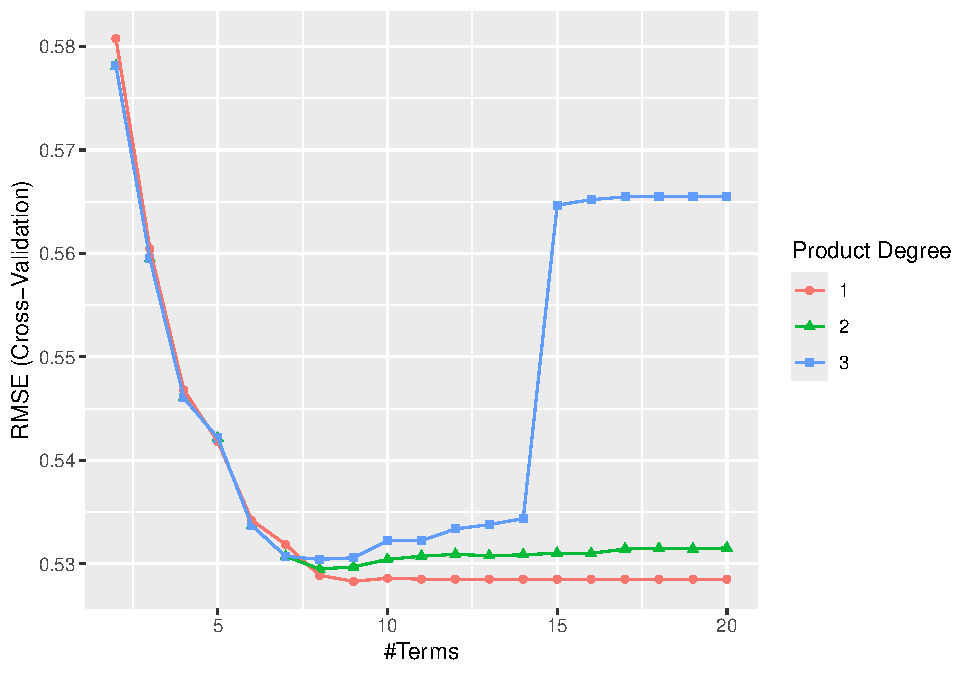
\includegraphics{p8106_midterm_project_files/figure-latex/unnamed-chunk-30-1.pdf}

\begin{Shaded}
\begin{Highlighting}[]
\NormalTok{mars.fit}\SpecialCharTok{$}\NormalTok{bestTune}
\end{Highlighting}
\end{Shaded}

\begin{verbatim}
##   nprune degree
## 8      9      1
\end{verbatim}

\begin{Shaded}
\begin{Highlighting}[]
\FunctionTok{coef}\NormalTok{(mars.fit}\SpecialCharTok{$}\NormalTok{finalModel)}
\end{Highlighting}
\end{Shaded}

\begin{verbatim}
##    (Intercept)    h(27.8-bmi)     h(time-57)     h(57-time)     genderMale 
##   10.847446930   -0.061997354   -0.002254182   -0.033529326   -0.296290451 
##      h(age-59)      h(59-age) smokingCurrent    h(bmi-23.7) 
##   -0.022957648    0.016138468   -0.205126851   -0.084380175
\end{verbatim}

\begin{Shaded}
\begin{Highlighting}[]
\FunctionTok{summary}\NormalTok{(mars.fit}\SpecialCharTok{$}\NormalTok{finalModel)}
\end{Highlighting}
\end{Shaded}

\begin{verbatim}
## Call: earth(x=matrix[5000,15], y=c(10.65,9.889,1...), keepxy=TRUE, degree=1,
##             nprune=9)
## 
##                coefficients
## (Intercept)      10.8474469
## genderMale       -0.2962905
## smokingCurrent   -0.2051269
## h(59-age)         0.0161385
## h(age-59)        -0.0229576
## h(bmi-23.7)      -0.0843802
## h(27.8-bmi)      -0.0619974
## h(57-time)       -0.0335293
## h(time-57)       -0.0022542
## 
## Selected 9 of 10 terms, and 5 of 15 predictors (nprune=9)
## Termination condition: RSq changed by less than 0.001 at 10 terms
## Importance: bmi, genderMale, time, age, smokingCurrent, raceAsian-unused, ...
## Number of terms at each degree of interaction: 1 8 (additive model)
## GCV 0.2787787    RSS 1384.431    GRSq 0.2166152    RSq 0.2216218
\end{verbatim}

\begin{Shaded}
\begin{Highlighting}[]
\CommentTok{\# we choose the relatively important variables to draw partial dependence plot}
\NormalTok{pdp1 }\OtherTok{=}\NormalTok{ pdp}\SpecialCharTok{::}\FunctionTok{partial}\NormalTok{(mars.fit, }\AttributeTok{pred.var =} \FunctionTok{c}\NormalTok{(}\StringTok{"bmi"}\NormalTok{), }\AttributeTok{grid.resolution =} \DecValTok{10}\NormalTok{) }\SpecialCharTok{|\textgreater{}} \FunctionTok{autoplot}\NormalTok{()}
\NormalTok{pdp2 }\OtherTok{\textless{}{-}}\NormalTok{ pdp}\SpecialCharTok{::}\FunctionTok{partial}\NormalTok{(mars.fit, }\AttributeTok{pred.var =} \FunctionTok{c}\NormalTok{(}\StringTok{"bmi"}\NormalTok{, }\StringTok{"time"}\NormalTok{), }\AttributeTok{grid.resolution =} \DecValTok{10}\NormalTok{) }\SpecialCharTok{|\textgreater{}}
\NormalTok{pdp}\SpecialCharTok{::}\FunctionTok{plotPartial}\NormalTok{(}\AttributeTok{levelplot =} \ConstantTok{FALSE}\NormalTok{, }\AttributeTok{zlab =} \StringTok{"log antibody"}\NormalTok{, }\AttributeTok{drape =} \ConstantTok{TRUE}\NormalTok{,}
\AttributeTok{screen =} \FunctionTok{list}\NormalTok{(}\AttributeTok{z =} \DecValTok{20}\NormalTok{, }\AttributeTok{x =} \SpecialCharTok{{-}}\DecValTok{60}\NormalTok{))}
\NormalTok{gridExtra}\SpecialCharTok{::}\FunctionTok{grid.arrange}\NormalTok{(pdp1, pdp2, }\AttributeTok{ncol =} \DecValTok{2}\NormalTok{)}
\end{Highlighting}
\end{Shaded}

\includegraphics{p8106_midterm_project_files/figure-latex/unnamed-chunk-34-1.pdf}

\paragraph{3.2.3 Generalized Additive Model
(GAM)}\label{generalized-additive-model-gam}

\begin{Shaded}
\begin{Highlighting}[]
\FunctionTok{set.seed}\NormalTok{(}\DecValTok{2}\NormalTok{)}
\NormalTok{gam.fit }\OtherTok{=} \FunctionTok{train}\NormalTok{(x, y, }\AttributeTok{method =} \StringTok{"gam"}\NormalTok{, }\AttributeTok{trControl =}\NormalTok{ ctrl1)}

\FunctionTok{summary}\NormalTok{(gam.fit)}
\end{Highlighting}
\end{Shaded}

\begin{verbatim}
## 
## Family: gaussian 
## Link function: identity 
## 
## Formula:
## .outcome ~ genderMale + raceAsian + raceBlack + raceHispanic + 
##     smokingFormer + smokingCurrent + diabetesYes + hypertensionYes + 
##     s(age) + s(sbp) + s(ldl) + s(bmi) + s(time) + s(height) + 
##     s(weight)
## 
## Parametric coefficients:
##                  Estimate Std. Error t value Pr(>|t|)    
## (Intercept)     10.228177   0.015328 667.269  < 2e-16 ***
## genderMale      -0.297837   0.014933 -19.945  < 2e-16 ***
## raceAsian       -0.003296   0.033009  -0.100    0.920    
## raceBlack       -0.010509   0.018837  -0.558    0.577    
## raceHispanic    -0.037424   0.026176  -1.430    0.153    
## smokingFormer    0.022219   0.016660   1.334    0.182    
## smokingCurrent  -0.193175   0.025834  -7.478  8.9e-14 ***
## diabetesYes      0.014230   0.020640   0.689    0.491    
## hypertensionYes -0.007678   0.015995  -0.480    0.631    
## ---
## Signif. codes:  0 '***' 0.001 '**' 0.01 '*' 0.05 '.' 0.1 ' ' 1
## 
## Approximate significance of smooth terms:
##                 edf Ref.df      F p-value    
## s(age)    9.908e-01      9 13.733  <2e-16 ***
## s(sbp)    6.175e-07      9  0.000   0.765    
## s(ldl)    6.648e-07      9  0.000   0.639    
## s(bmi)    4.179e+00      9 41.897  <2e-16 ***
## s(time)   7.892e+00      9 44.960  <2e-16 ***
## s(height) 1.234e+00      9  0.278   0.121    
## s(weight) 2.262e-06      9  0.000   0.666    
## ---
## Signif. codes:  0 '***' 0.001 '**' 0.01 '*' 0.05 '.' 0.1 ' ' 1
## 
## R-sq.(adj) =   0.22   Deviance explained = 22.4%
## GCV = 0.27867  Scale est. = 0.27738   n = 5000
\end{verbatim}

\begin{Shaded}
\begin{Highlighting}[]
\NormalTok{gam.fit}\SpecialCharTok{$}\NormalTok{bestTune}
\end{Highlighting}
\end{Shaded}

\begin{verbatim}
##   select method
## 2   TRUE GCV.Cp
\end{verbatim}

\begin{Shaded}
\begin{Highlighting}[]
\NormalTok{gam.fit}\SpecialCharTok{$}\NormalTok{finalModel}
\end{Highlighting}
\end{Shaded}

\begin{verbatim}
## 
## Family: gaussian 
## Link function: identity 
## 
## Formula:
## .outcome ~ genderMale + raceAsian + raceBlack + raceHispanic + 
##     smokingFormer + smokingCurrent + diabetesYes + hypertensionYes + 
##     s(age) + s(sbp) + s(ldl) + s(bmi) + s(time) + s(height) + 
##     s(weight)
## 
## Estimated degrees of freedom:
## 0.991 0.000 0.000 4.179 7.892 1.234 0.000 
##  total = 23.3 
## 
## GCV score: 0.2786734
\end{verbatim}

\paragraph{3.2.4 Model Comparison
(resampling)}\label{model-comparison-resampling-1}

\begin{Shaded}
\begin{Highlighting}[]
\NormalTok{comparison }\OtherTok{=} \FunctionTok{resamples}\NormalTok{(}\FunctionTok{list}\NormalTok{(}\AttributeTok{MARS =}\NormalTok{ mars.fit, }\AttributeTok{GAM =}\NormalTok{ gam.fit))}
\FunctionTok{summary}\NormalTok{(comparison)}
\end{Highlighting}
\end{Shaded}

\begin{verbatim}
## 
## Call:
## summary.resamples(object = comparison)
## 
## Models: MARS, GAM 
## Number of resamples: 10 
## 
## MAE 
##           Min.   1st Qu.    Median      Mean   3rd Qu.      Max. NA's
## MARS 0.4120189 0.4180233 0.4203065 0.4224208 0.4285348 0.4360995    0
## GAM  0.4127242 0.4190075 0.4202804 0.4224455 0.4273258 0.4352565    0
## 
## RMSE 
##           Min.   1st Qu.    Median      Mean   3rd Qu.      Max. NA's
## MARS 0.5066327 0.5230870 0.5316602 0.5282995 0.5354905 0.5457286    0
## GAM  0.5091877 0.5223782 0.5306669 0.5279212 0.5336806 0.5451253    0
## 
## Rsquared 
##           Min.   1st Qu.    Median      Mean   3rd Qu.      Max. NA's
## MARS 0.1766328 0.1941155 0.2028183 0.2159220 0.2369173 0.2730827    0
## GAM  0.1795042 0.1955023 0.2071224 0.2170567 0.2376473 0.2735385    0
\end{verbatim}

\paragraph{3.1.6 Test Set Performance}\label{test-set-performance-1}

\begin{Shaded}
\begin{Highlighting}[]
\CommentTok{\# Make predictions using each mode}
\NormalTok{pred\_ss }\OtherTok{=} \FunctionTok{predict}\NormalTok{(fit.ss, }\AttributeTok{x =}\NormalTok{ dat2}\SpecialCharTok{$}\NormalTok{bmi)}
\NormalTok{pred\_mars }\OtherTok{=} \FunctionTok{predict}\NormalTok{(mars.fit, }\AttributeTok{newdata =}\NormalTok{ x\_test)}
\NormalTok{pred\_gam }\OtherTok{=} \FunctionTok{predict}\NormalTok{(gam.fit, }\AttributeTok{newdata =}\NormalTok{ x\_test)}

\NormalTok{mse\_ss }\OtherTok{=} \FunctionTok{mean}\NormalTok{((dat2}\SpecialCharTok{$}\NormalTok{log\_antibody }\SpecialCharTok{{-}}\NormalTok{ pred\_ss}\SpecialCharTok{$}\NormalTok{y)}\SpecialCharTok{\^{}}\DecValTok{2}\NormalTok{)}
\NormalTok{mse\_mars }\OtherTok{=} \FunctionTok{mean}\NormalTok{((y\_test }\SpecialCharTok{{-}}\NormalTok{ pred\_mars)}\SpecialCharTok{\^{}}\DecValTok{2}\NormalTok{)}
\NormalTok{mse\_gam }\OtherTok{=} \FunctionTok{mean}\NormalTok{((y\_test }\SpecialCharTok{{-}}\NormalTok{ pred\_gam)}\SpecialCharTok{\^{}}\DecValTok{2}\NormalTok{)}

\NormalTok{test\_performance\_non\_linear }\OtherTok{\textless{}{-}} \FunctionTok{data.frame}\NormalTok{(}
  \AttributeTok{Model =} \FunctionTok{c}\NormalTok{(}\StringTok{"Smoothing Spline"}\NormalTok{, }\StringTok{"MARS"}\NormalTok{, }\StringTok{"GAM"}\NormalTok{),}
  \AttributeTok{Test\_ERROR =} \FunctionTok{c}\NormalTok{(mse\_ss, mse\_mars, mse\_gam)}
\NormalTok{)}
\FunctionTok{print}\NormalTok{(test\_performance\_non\_linear)}
\end{Highlighting}
\end{Shaded}

\begin{verbatim}
##              Model Test_ERROR
## 1 Smoothing Spline  0.3584620
## 2             MARS  0.2838458
## 3              GAM  0.3249953
\end{verbatim}

\subsubsection{4. Model Comparison between Linear and non-linear
Models}\label{model-comparison-between-linear-and-non-linear-models}

\begin{Shaded}
\begin{Highlighting}[]
\CommentTok{\# MSE comparison}

\NormalTok{test\_mse\_table }\OtherTok{=} \FunctionTok{data.frame}\NormalTok{(}
  \AttributeTok{Model =} \FunctionTok{c}\NormalTok{(}\StringTok{"Linear Regression"}\NormalTok{, }\StringTok{"Ridge Regression"}\NormalTok{, }\StringTok{"Lasso Regression"}\NormalTok{, }
            \StringTok{"Elastic Net Regression"}\NormalTok{,}\StringTok{"Smoothing Spline"}\NormalTok{, }\StringTok{"MARS"}\NormalTok{, }\StringTok{"GAM"}\NormalTok{),}
  \AttributeTok{MSE =} \FunctionTok{c}\NormalTok{(lm.test.error,ridge.test.error,}
\NormalTok{          lasso.test.error, mse\_ss, enet.test.error, }
\NormalTok{          mse\_mars, mse\_gam)}
\NormalTok{) }\SpecialCharTok{|\textgreater{}} \FunctionTok{arrange}\NormalTok{(MSE)}

\FunctionTok{kable}\NormalTok{(test\_mse\_table, }\AttributeTok{sort =} \ConstantTok{TRUE}\NormalTok{)}
\end{Highlighting}
\end{Shaded}

\begin{longtable}[]{@{}lr@{}}
\toprule\noalign{}
Model & MSE \\
\midrule\noalign{}
\endhead
\bottomrule\noalign{}
\endlastfoot
MARS & 0.2838458 \\
Linear Regression & 0.3229854 \\
Smoothing Spline & 0.3247256 \\
GAM & 0.3249953 \\
Ridge Regression & 0.3258077 \\
Lasso Regression & 0.3288173 \\
Elastic Net Regression & 0.3584620 \\
\end{longtable}

The best model is the MARS model with the smallest test error.

\end{document}
